\documentclass[letter,12pt]{book}
\usepackage[utf8]{inputenc}
\usepackage{graphicx}
\usepackage[spanish]{babel}
\usepackage[margin=2cm]{geometry}

\begin{document}

\author{Carlos Toledo Silva		C-311\\Aylín Álvarez Santos		C-312\\Rocio Ortíz Gancedo		C-311\\Ariel Alfonso Triana Pérez 		C-311}
\title{Proyecto de desarrollo: Cine+}
\date{2021}

\makeatletter

% Portada
\begin{titlepage}
\centering

\vspace{5cm}

{ \Huge \textbf{\@title}}

\vspace{5cm}


\includegraphics[width=6cm]{./img/logo-matcom.jpg}

\vspace{5cm}

\textbf{Equipo de desarrollo:}

 \@author

\vspace{1cm}

\@date
\end{titlepage}

% Tabla de contenidos
\tableofcontents


\mainmatter
\chapter{Introducción}

\section{Alcance del producto}

N/A

\section{Descripción general}

\subsection{Perspectiva del producto}

El producto busca controlar la venta de entradas de un cine denominado Cine+. Para esto el producto debe dar soporte tanto a la venta de entradas por taquillas como a la venta de entradas por internet, garantizándose la coordinación de las mismas.

\subsection{Funciones del Producto}

El producto es una aplicación web multiplataforma que permite la compra de entradas a través de su página web por parte de los clientes y calcula el costo de la entradas atendiendo a diferentes parámetros. Además da soporte a la inscripción de usuarios como socios del club de Cine+, así como los beneficios de los que estos pueden disfrutar. También el producto permite la anulación de las compras de entradas por parte de los usuarios y hace las actualizaciones pertinentes dada la anulación. El producto permite además que los gerentes del cine puedan actualizar el listado de películas y horarios disponibles y que estos sean mostrados en la web. Además estos pueden consultar las estadísticas de venta de entradas por diferentes parámetros. También se posibilita la visualización en una página web de las 10 películas sugeridas por uno de los gerentes del cine.

\subsection{Características de los usuarios}

Con el producto interactuarán tres tipos de usuarios: clientes, taquilleros y gerentes. Los gerentes dominan toda la información relacionada con la puesta en escena de las peliculas: horarios, precios, películas que se mostrarán, sugerencias, etc. Los taquilleros dominan como controlar el sistema de tal forma que la venta de entrada puedea mantenerse coordinada entre la venta física en la taquilla y la venta web. Los 3 tipos de usuarios están identificados tanto con dispositivos móviles y tabletas como con computadoras.

Los gerentes y taquilleros tienen el conocimiento necesario para operar este tipo de aplicación web realizando sus respectivas funciones. Los clientes conforman un grupo muy heterogéneo, algunos no tienen conocimiento con productos similares, ahí la necesidad de que la interfaz con la que interactúan sea cómoda.

\subsection{Restricciones Generales}

El cliente solicita que el sistema en cuestión sea una aplicación web, con las funcionalidades anteriormente mencionadas. Además informa que ya reservaron el hosting y dominio (www.cine+.com) de la página y la base de datos. El hosting tiene 4000 MB de almacenamiento.

El cliente pide que las páginas carguen en el tiempo recomendado por los expertos en posicionamiento SEO, para el posicionamiento en buscadores como Google o Bing. Además que el sitio tenga un flujo de navegación sencillo, y que la navegación no sobrepase el tercer nivel.

\section{Resumen del resto del documento}

En el Cap\'itulo 2 nos referiremos a los requerimientos espec\'ificos del producto, por lo que abordaremos sus requerimientos funcionales, no funcionales y de entorno. En el Cap\'itulo 3 abundaremos en las diferentes funcionalidades de la aplicaci\'on y se explicar\'a como ocurre la interacci\'on entre los diferentes tipos de usuarios y el producto.

El el Cap\'itulo 4 comentaremos sobre la metodolog\'ia seleccionada y daremos argumentos del porqu\'e de su elecci\'on. Adem\'as nos referiremos a los principios que seguimos para el desarrollo de la aplicaci\'on. En el Cap\'itulo 5 mencionaremos la arquitectura utilizada y expondremos los motivos de la elecci\'on de dicha arquitectura por encima de otras que tambi\'en fueron analizadas.

En el cap\'itulo 6 abordaremos tanto los patrones de visualizaci\'on de datos como los patrones de acceso a datos empleados en el desarrollo del producto. Finalmente en el cap\'itulo 7 estaremos viendo la modelaci\'on de la base de datos.
\chapter{Requerimientos Específicos}\label{ch:req}

\section{Requerimientos funcionales}

El sitio web debe permitir que cualquier usuario pueda comprar entradas. Para ello debe buscar la película deseada y mostrar los horarios y salas en que estará en pantalla dicha película. Luego de que el usuario escoja la sala y el horario de su preferencia, el sistema le pregunta al usuario el número de entradas y asigna unas butacas autómaticamente, pero da opción a que el usuario las modifique a su gusto, las cuales pasarán a estar reservadas de forma provisional. Si pasado algún un tiempo (por defecto 10 min) el usuario no ha efectuado la compra o éste la cancela las butacas vuelven a estar disponibles.

Para el cálculo del precio de la entrada, se deben tener en cuenta los diferentes descuentos que se ofrecen.

Los usuarios que los deseen puden darse de alta como socios del club Cine+, cumpliendo con las pasos pertinentes. A cada socio, cada vez que compre una entrada, se le sumarán 5 puntos, los cuales podrá cambiar en el futuro por entradas. Para hacer esto el socio deberá contar con la suficiente cantidad de puntos para poder pagar todas las entradas de su compra. El precio de la entrada es de 20 puntos por defecto, aunque este se podrá configurar.

La compra por web se realiza por medio de tarjeta de crédito, utilizándose una pasarela de pago segura. En taquilla se admite sólo pago en efectivo. Además se debe poder imprimir un comprobante de venta de las entradas.

Una compra realizada a través de la web puede ser anulada hasta 2 horas antes del comienzo  de la sesión, restableciéndole al cliente el costo de la compra y dejando sus butacas disponibles. Si el pago fue hecho por un socio utilizando sus puntos, estos serán devueltos a su cuenta.

Los gerentes podrán actualizar el listado de películas y los horarios, los cuales serán mostrados en el sittio. Además estos podrán consultar estadísticas sobre las ventas de entradas.

Se exige mostrar una vista de 10 películas sugeridas para ver, la cual será actualizada periódicamente. Estará lista seguirá un criterio escogido por alguno de los gerentes.

\section{Requerimientos no funcionales}

Dado que esta es una aplicación web para la venta de entradas para un cine, se le debe dar bastante información sobre el tema a la aplicación para que un navegador pueda encontrala más rápidamente.

Los datos referentes a las películas (salas, horarios, etc) serán guardados en una base de datos SQLite. En esta se guardará además la información referente a los socios, taquilleros y a los gerentes del cine.

El acceso de los gerentes, los taquilleros y los socios de Cine+ al sistema es a través del nombre de usuario y contraseña. Para el acceso al perfil de usuario es necesario comunicaciones seguras, así como para navegar en la administración para el caso de los gerantes y gestionar las ventas para el caso de los taquilleros. Las mismas también son necesarias para la realización de los pagos mediante la pasarela. Por lo anterior es necesario contratar un certificado SSL para el sitio. En caso de que se acceda a través de HTTP será imposible ingresar  el nombre y la contraseña, así como recuperar contraseñas.

La interfaz del usuario deberá ser tan familiar como sea posible a los usuarios, lo cual dependerá de la experiencia de los mismos en el uso de otras aplicaciones web. Se agregará además una documentación online para los clientes, para los taquilleros y  para los gerentes; donde además la dedicada a los clientes contará con información referente sobre cómo convertirse en un socio de Cine+ y los beneficios que trae serlo.

\section{Requerimientos de Entorno}

Aunque los gerentes y taquilleros del cine pueden poseer una variada gama de dispositivos electrónicos se conece que la administración de Cine+ les proverá de recursos necesarios para la realización de sus funciones. Dicho esto se tiene la seguridad de que cada gerente o taquillero tiene asignado uno de estos dos dispositivos para el acceso:

\begin{enumerate}
    \item Laptop ASUS con procesador Intel Core i7 de 4ta generación con navegador Mozilla Firefox 86.0
    \item Laptop HP con procesador Intel Core i5 de 8va generación con navegador Google Chrome 88.0.4324.104
\end{enumerate}

Además en caso de que el gerente no posea un dispositivo móvil de al menos gama media con el que pueda realizar sus funciones, la administración le proverá de un Samsung Galaxy A10 con conexión a Internet y navegadores como Google Chrome 89.0.4389.72 y Safari 14.0.2. 

Los clientes como se conoce son una masa de usuarios heterogénea, como también lo es la masa de dispositivos que ellos tienen disponibles: laptops, móviles, tabletas todos con distintos tipos de sistemas operativos (Windows, Linux, iOS y Android en distintas versiones). Además, en este grupo de usuarios existen distintos tipos de navegadores como Mozilla Firefox, Google Chrome, Opera, Microsoft Edge, Brave, en distintas versiones de los mismos.

En cuanto al hosting, el cliente tiene disponible uno con Windows Server, con 4000 MB de almacenamiento, 1000 MB de base de datos en SQLite, 1 cuenta de acceso para administración, 1000 conexiones concurrentes, 3 cuentas FTP, 1024 Kbps de velocidad de transferencia, soporte para Javascript, para ASP.NET. La aplicación web se desarrollará sobre .NET 5, y C\#.

Para el servidor se tiene un Intel(R) Core(TM) i7-8250U CPU 2.60 GHz, 2.60 GHz, con 16GB RAM. El servidor con arquitectura física de 64 bit.

\chapter{Funcionalidades del producto}

\chapter{Enfoque Metodológico}

Para el desarrollo de este proyecto se aplicará la metodología ágil Extreme Programming (XP). 

Se seleccionó una metodología ágil debido a los beneficios de estas y la adaptabilidad a las características de nuestro problema. Una de sus ventajas es que facilita la planificación debido a la división de proyectos en sprints, siendo mas sencillo para el desarrollador abordar el proyecto en pequeñas fases con una duración y alcance determinados. El aumento de la implicación y de la motivación del equipo constituye otra ventaja, puesto que todos los miembros del equipo están informados del estado del proyecto. El cliente desde las primeras etapas del proyecto se le entrega un producto mínimo viable, por lo que este no debe esperar mucho tiempo para empezar a recuperar la inversión realizada. Las entregas continuas garantizan que tras la finalización de cada sprint el software se actualiza con nuevas modificaciones, mejora la calidad del producto debido a los testeos que se realizan después de la finalización de cada fase de desarrollo. La flexibilidad antes los cambios es otra de las características mas importantes ya que permite adaptación del proyecto a las nuevas necesidades o imprevistos que puedan surgir. 

Entre el grupo de metodologías ágiles se seleccionó la metodología XP de acuerdo a las características y ventajas de esta sobre nuestro problema.

Una de estas características que nos llevó a escoger esta metodología y no Scrum es debido a los requisitos del cliente. Se planean reuniones cada 15 días donde se entrega los avances del producto y un informe adjunto sobre el trabajo realizado en esos días, no se planean reuniones diarias, aunque  contamos con la disponibilidad del cliente para todos los encuentros en los que sea necesario debatir y valorar las sugerencias que brinde nuestro equipo y el cliente para lograr simplicidad, lo cual propicia la retroalimentación frecuente entre ambas partes, lo cual es una práctica de la metodología escogida (Cliente in-situ).

El trabajo se realizará en parejas lo cual constituye una principal característica la metodología XP, teniendo como gran ventaja la detección de errores conforme son introducidos en el código (inspecciones de código continuas), por consiguiente, la tasa de errores del producto final es más baja, los diseños son mejores y el tamaño del código menor (continua discusión de ideas de los programadores), varias personas entienden las diferentes partes sistema.

El listado de los requisitos del proyecto en cuestión se encuentra bien detallado, pero debido a la inexperiencia del personal, el desarrollo de este puede sufrir cambios por lo que el empleo de esta metodología facilitará la asimilación de estos. 

El personal tiene como principio hacer un software de calidad, en el que se apliquen los principios SOLID, DRY, KISS, YAGNI, una arquitectura que permita el desacoplamiento y extensibilidad, además que constituye una exigencia del cliente. De esta manera pondríamos en práctica la refactorización y el diseño simple.

Como característica del personal se permite que cualquier programador puede cambiar cualquier parte del código en cualquier momento motivando a la aparición de nuevas ideas por parte del personal. 

Cada uno de los motivos anteriores expuestos conllevó a la utilización de esta metodología ante el resto de metodologías ágiles en el proyecto asignado.

\chapter{Arquitectura}

Luego del análisis de los requerimientos y las funcionalidades que solicita el cliente en el producto final, se necesita determinar la arquitectura más adecuada para el software a implementar. Se analizaron las siguientes arquitectura para implementarlas en el proyecto:

\begin{enumerate}
    \item[$\bullet$] Arquitectura en Capas, conocida en inglés como N-Layered, y tiene variantes como Onion Layered o Hexagonal Layered
    \item[$\bullet$] Arquitectura orientada a Microservicios
    \item[$\bullet$] Arquitectura orientada a Servicios, o SOA por sus siglas en inglés.
\end{enumerate}

\section{Arquitectura seleccionada}

Se analizaron las tres arquitecturas antes mencionadas buscando la que mejor se ajuste a los requerimientos del proyecto, y que permita el desacoplamiento, la extensibilidad, la escalabilidad, el mantenimiento y el proceso de testing. 

Al analizar la arquitectura N-Layered con sus variantes, se nota que a pesar de su simplicidad y sus facilidades de implementación en pequeños proyectos, su proceso de testing es muy complicado. Por ejemplo si se introduce un cambio en alguna de las líneas del código, es necesario volver a invertir tiempo en ejecutar todo el Unit Testing. Dada su implementación monolítica, entonces se cumple que su escalabilidad, y mantenimiento son muy complejos. Por tanto, se considera que no es una de las mejores opciones para aplicar en el proyecto.

Al analizar las otras arquitecturas se obtuvieron mejores resultados a pesar de tener puntuaciones más altas en complejidad y en costos de implementación. Por eso se decidió, que dado el corto tiempo para la implementación del software, tampoco serían buenas opciones.

Por tanto, se desarrolló una arquitectura que es el resultado de mezclar la arquitectura en capas y la arquitectura de microservicios, con el fin de obtener la simplicidad de la implementación, mantener costes de implementación relativamente bajos y lograr escalabilidad, mantenimiento, extensibilidad y desacoplamiento.

\chapter{Patrones de visualización y de datos}
\chapter{Modelo de datos}\label{ch:model}

\begin{figure}[h]
    \begin{center}
        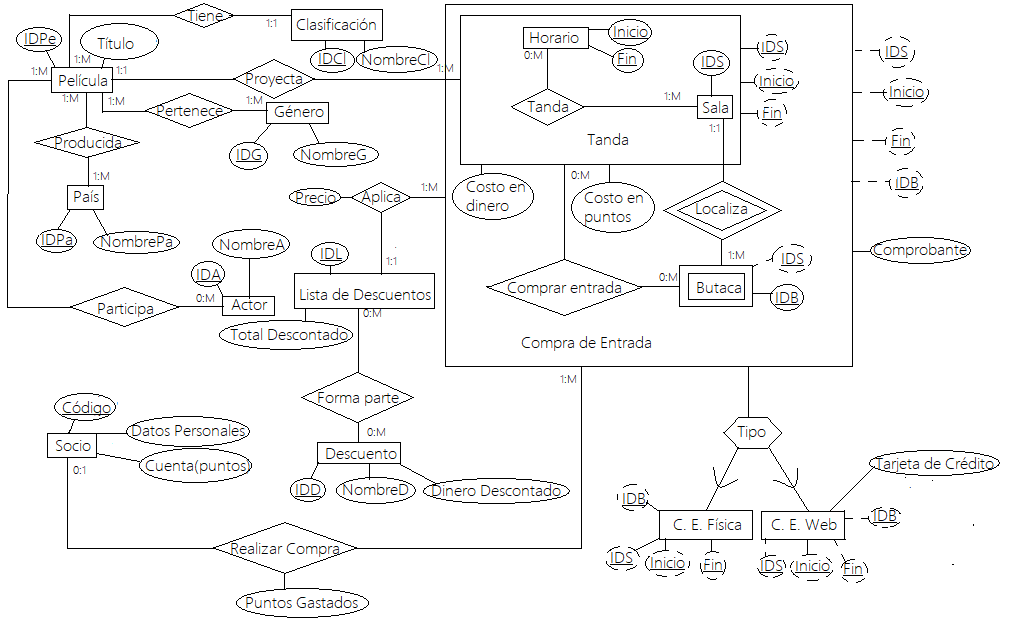
\includegraphics[width=16.0cm]{./chapters/img/is.png}
    \end{center}

    \caption{MERX de la modelación conceptual de la base de datos.}
\end{figure}

A partir de esta modelación se obtiene la siguiente descomposición que cumple la Propiedad de Preservación de las Dependencias Funcionales (PPDF) y la Propiedad del Join sin Pérdida de información  y cada uno de sus esquemas relacionales se encuentra en 3ra Forma Normal.\\
	
	$U_{Pelicula}=\{IDPe, Titulo\}$
	
	$F_{Pelicula}=\{IDPe\rightarrow Titulo\}$\\
	
	$U_{Pais}=\{IDPa, NombrePa\}$
	
	$F_{Pais}=\{IDPa\rightarrow NombrePa\}$\\
	
	$U_{G\acute{e}nero}=\{IDG, NombreG\}$
	
	$F_{G\acute{e}nero}=\{IDG\rightarrow NombreG\}$\\
	
	$U_{Actor}=\{IDA, NombreA\}$
		
	$F_{Actor}=\{IDA\rightarrow NombreA\}$\\
	
	$U_{Horario}=\{Inicio, Fin\}$
		
	$F_{Horario}=\emptyset$\\
	
	$U_{Sala}=\{IDS\}$
	
	$F_{Sala}=\emptyset$\\
	
	$U_{Butaca}=\{IDS,IDB\}$
		
	$F_{Butaca}=\emptyset$\\
	
	$U_{Tanda}=\{IDS, Inicio, Fin, Costo~en~dinero, Costo~en~puntos, IDPe\}$
	
	$F_{Proyecta}=\{IDS, Inicio, Fin\rightarrow Costo~en~dinero, Costo~en~puntos, IDPe\}$\\
	
	$U_{Descuento}=\{IDD, NombreD, DineroDescontado\}$
		
	$F_{Descuento}=\{IDD\rightarrow NombreD, Dinero~Descontado\}$\\
	
	$U_{Lista~de~Descuentos}=\{IDL,Total~Descontado\}$
		
	$F_{Lista~de~Descuentos}=\{IDL\rightarrow Total~Descontado\}$\\
	
	$U_{Compra~de~Entrada}=\{IDS, Inicio, Fin, IDB, IDL, Precio, Comprobante\}$
		
	$F_{Compra~de~Entrada}=\{IDS, Inicio, Fin,IDB\rightarrow IDL, Precio, Comprobante\}$\\
	
	$U_{Socio}=\{C\acute{o}digo,Datos~Personales,Cuenta(puntos)\}$
		
	$F_{Socio}=\{C\acute{o}digo\rightarrow Datos~Personales,Cuenta(puntos)\}$\\
	
	$U_{Realizar~Compra}=\{IDS,Inicio,Fin,IDB,C\acute{o}digo,Puntos~Gastados\}$
		
	$F_{Realizar~Compra}=\{IDS,Inicio,Fin,IDB\rightarrow C\acute{o}digo,Puntos~Gastados\}$\\
	
	$U_{C.E~Fisica}=\{IDS,Inicio,Fin,IDB\}$
		
	$F_{C.E. Fisica}=\emptyset$\\
	
	$U_{C.E~Web}=\{IDS,Inicio,Fin,IDB,Tarjeta~de~Cr\acute{e}dito\}$
		
	$F_{C.E~Web}=\{IDS,Inicio,Fin,IDB\rightarrow Tarjeta~de~Cr\acute{e}dito\}$\\
		
	$U_{Producida}=\{IDPe,IDPa\}$
		
	$F_{Producida}=\emptyset$\\
	
	$U_{Participa}=\{IDPe,IDA\}$
		
	$F_{Participa}=\emptyset$\\
	
	$U_{Forma~Parte}=\{IDL,IDD\}$
		
	$F_{Forma~Parte}=\emptyset$\\
	
	$U_{Producida}=\{IDPe,IDPa\}$
		
	$F_{Producida}=\emptyset$\\
	
	$U_{Pertence}=\{IDPe,IDPa\}$
		
	$F_{Pertenece}=\emptyset$\\
		
	$\rho=(Pelicula,Pais,G\acute{e}nero,Actor,Horario,Sala,Tanda,Butaca,Proyecto,Descuento,$
	
	$Lista~de~Descuentos,Compra~de~Entrada,Socio,Realizar~Compra,C.E.Fisica,C.E.Web,Producida,$
	
	$Participa,Forma~Parte,Pertenece)$	
\appendix
\chapter{Manual de Usuario}
\section{Registro e ingreso de cuentas de usuarios}

Para el ingreso de cuentas de usuarios  se tiene el siguiente formulario para todos los usuarios, donde es necesario que se introduzca el nombre de usuario registrado y la contraseña del mismo. La página de ingreso se muestra a continuación:\\

\begin{figure}[h!]
	\centering
	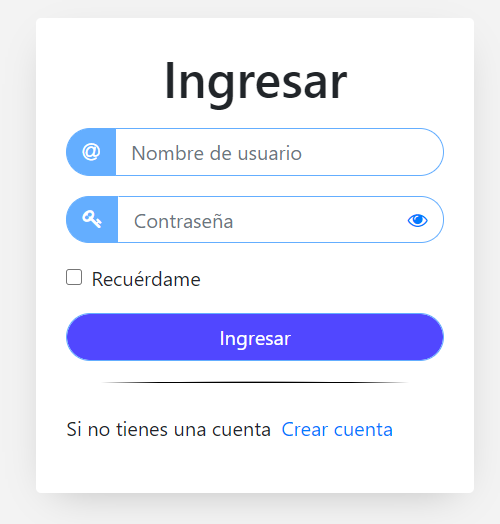
\includegraphics[width=7cm]{./chapters/img/login.png}
	
	\label{fig:login}
	\caption{Login}
\end{figure}

En caso de que las credenciales del usuario sean correctas esta página redireccionará a la página de inicio del sistema que se muestra a continuación:\\

\begin{figure}[h!]
	\centering
	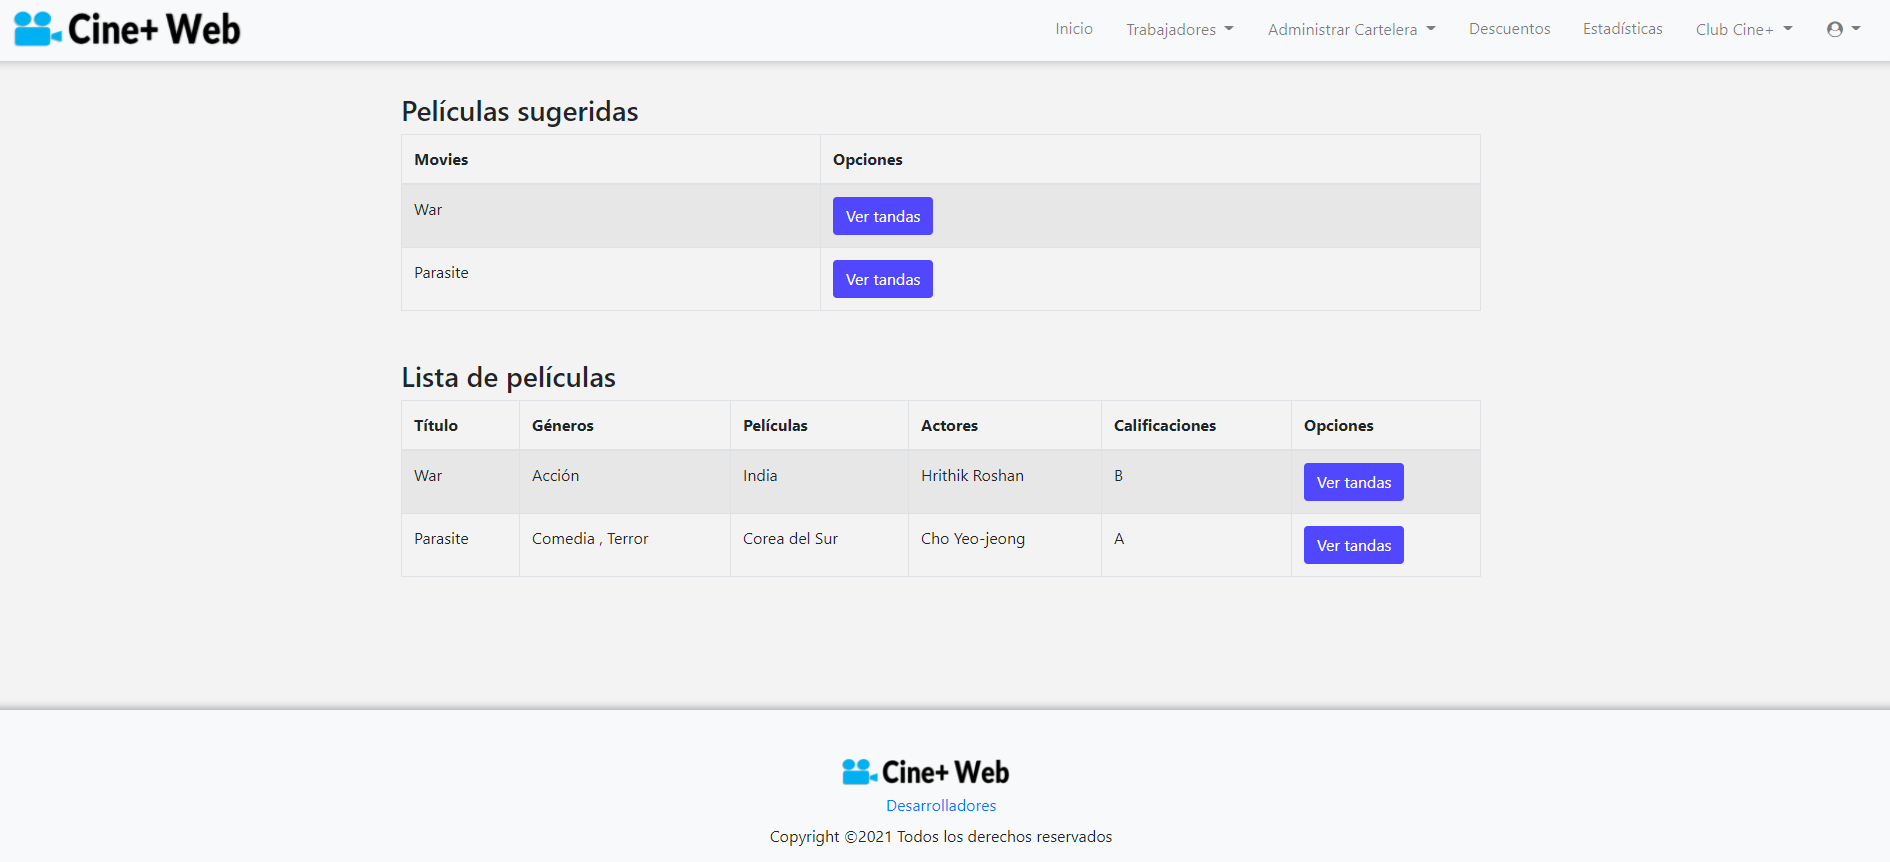
\includegraphics[scale=0.35]{./chapters/img/Index.png}
	
	\label{fig:Index}
	\caption{P\'agina Inicial}
\end{figure}
\newpage

Como se observa en la página de Inicio se tiene una cabecera que está presente en todas las páginas. En la cabecera estará todas las páginas a las que puede acceder un usuario en dependencia de sus permisos.\\

A continuación se presentan las cabeceras de los tres (3) tipos de usuarios:\\

\begin{figure}[h!]
	\centering
	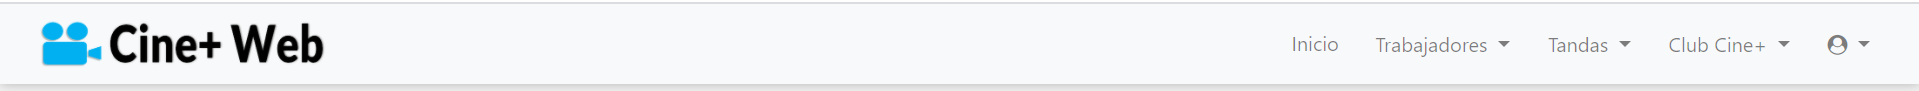
\includegraphics[scale=0.4]{./chapters/img/header_admin.png}
	
	\label{fig:header_admin}
	\caption{Cabecera Gegerente}
\end{figure}
\begin{figure}[h!]
	\centering
	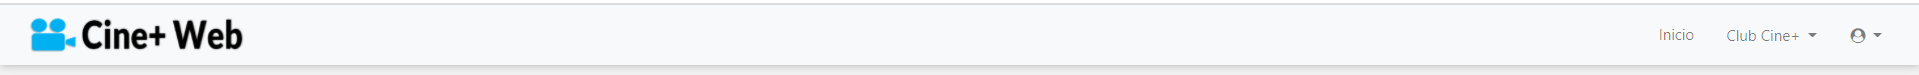
\includegraphics[scale=0.4]{./chapters/img/header_taquillero.png}
	
	\label{fig:header_taquillero}
	\caption{Cabecera Taquillero}
\end{figure}
\begin{figure}[h!]
	\centering
	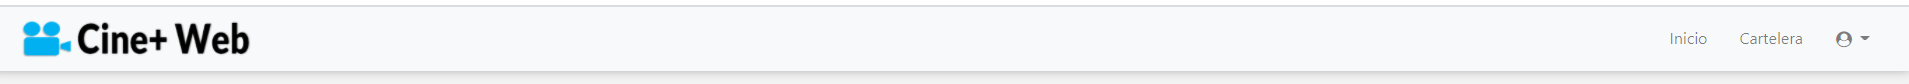
\includegraphics[scale=0.4]{./chapters/img/header_client.png}
	
	\label{fig:header_client}
	\caption{Cabecera Cliente}
\end{figure}


Para el registro de usuarios se tiene el siguiente formulario accesible desde la cabecera de los usuarios que no están autenticados.
\newpage

\begin{figure}[h!]
	\centering
	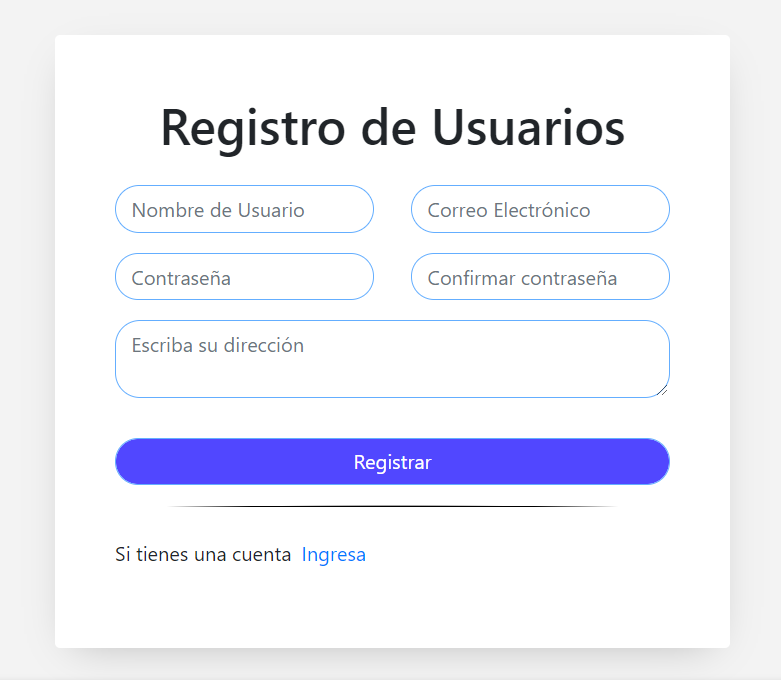
\includegraphics[scale=0.4]{./chapters/img/register.png}
	
	\label{fig:register}
	\caption{Registro}
\end{figure}

Los gerentes son los que est\'an facultados para la designación de nuevos taquilleros y gerentes. Para ello se cuenta con un formulario similar al de registro de usuarios accesible desde \verb|Trabajadores|, opci\'on \verb|Gerentes| y \verb|Taquilleros| disponible en la cabecera de los usuarios con el rol de gerente.\\

Los taquilleros tiene como tarea la venta de entrada en taquilla y la gestion de cuentas de socio.

\subsection{Gestión de Cartelera}

Todas las opciones referentes a la gestión de cartelera est\'an disponibles en las cabeceras en la pesta\~na \verb*|Administar| \verb*|Cartelera|.\\

\begin{figure}[h!]
	\centering
	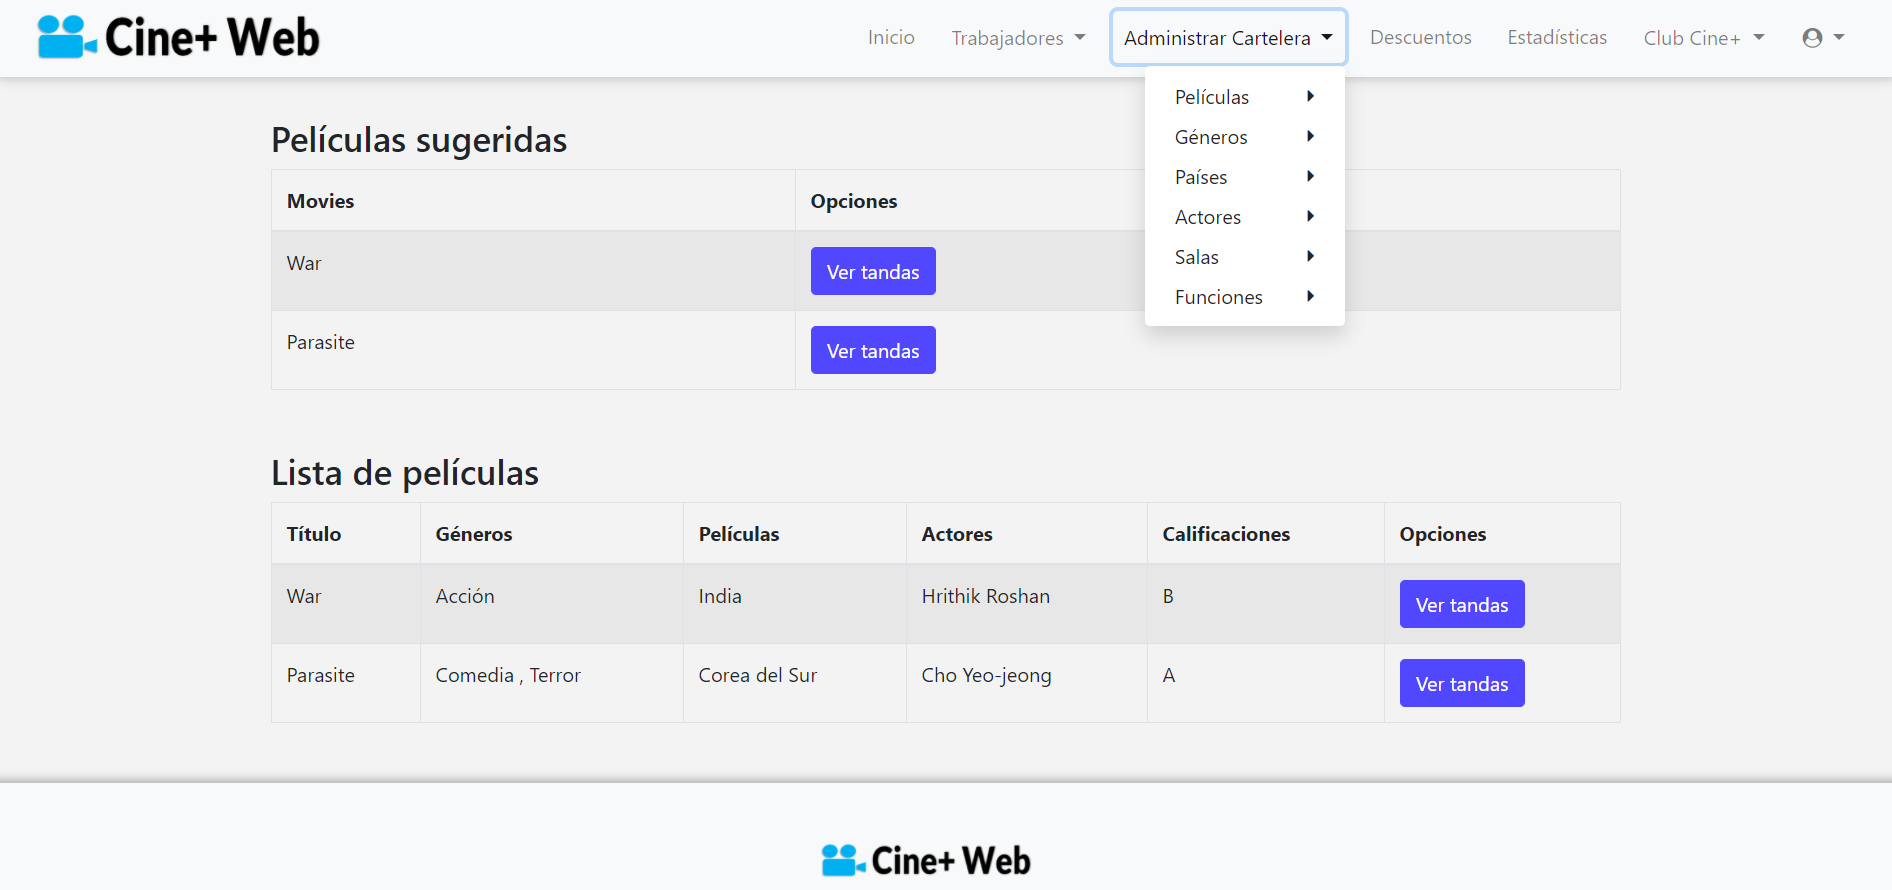
\includegraphics[scale=0.35]{./chapters/img/cartelera.png}
	
	\label{fig:cartelera}
	\caption{Administrar Cartelera}
	
\end{figure}

\subsubsection{Gestor de Pel\'iculas}
La opci\'on referente a la gesti\'on de pel\'iculas es accesible desde la pesta\~na \verb*|Administar| \verb*|Cartelera|. Al hacer click se despliegan dos opciones referentes a pel\'iculas como se observa en la siguiente imagen.

\newpage
\begin{figure}[h!]
	\centering
	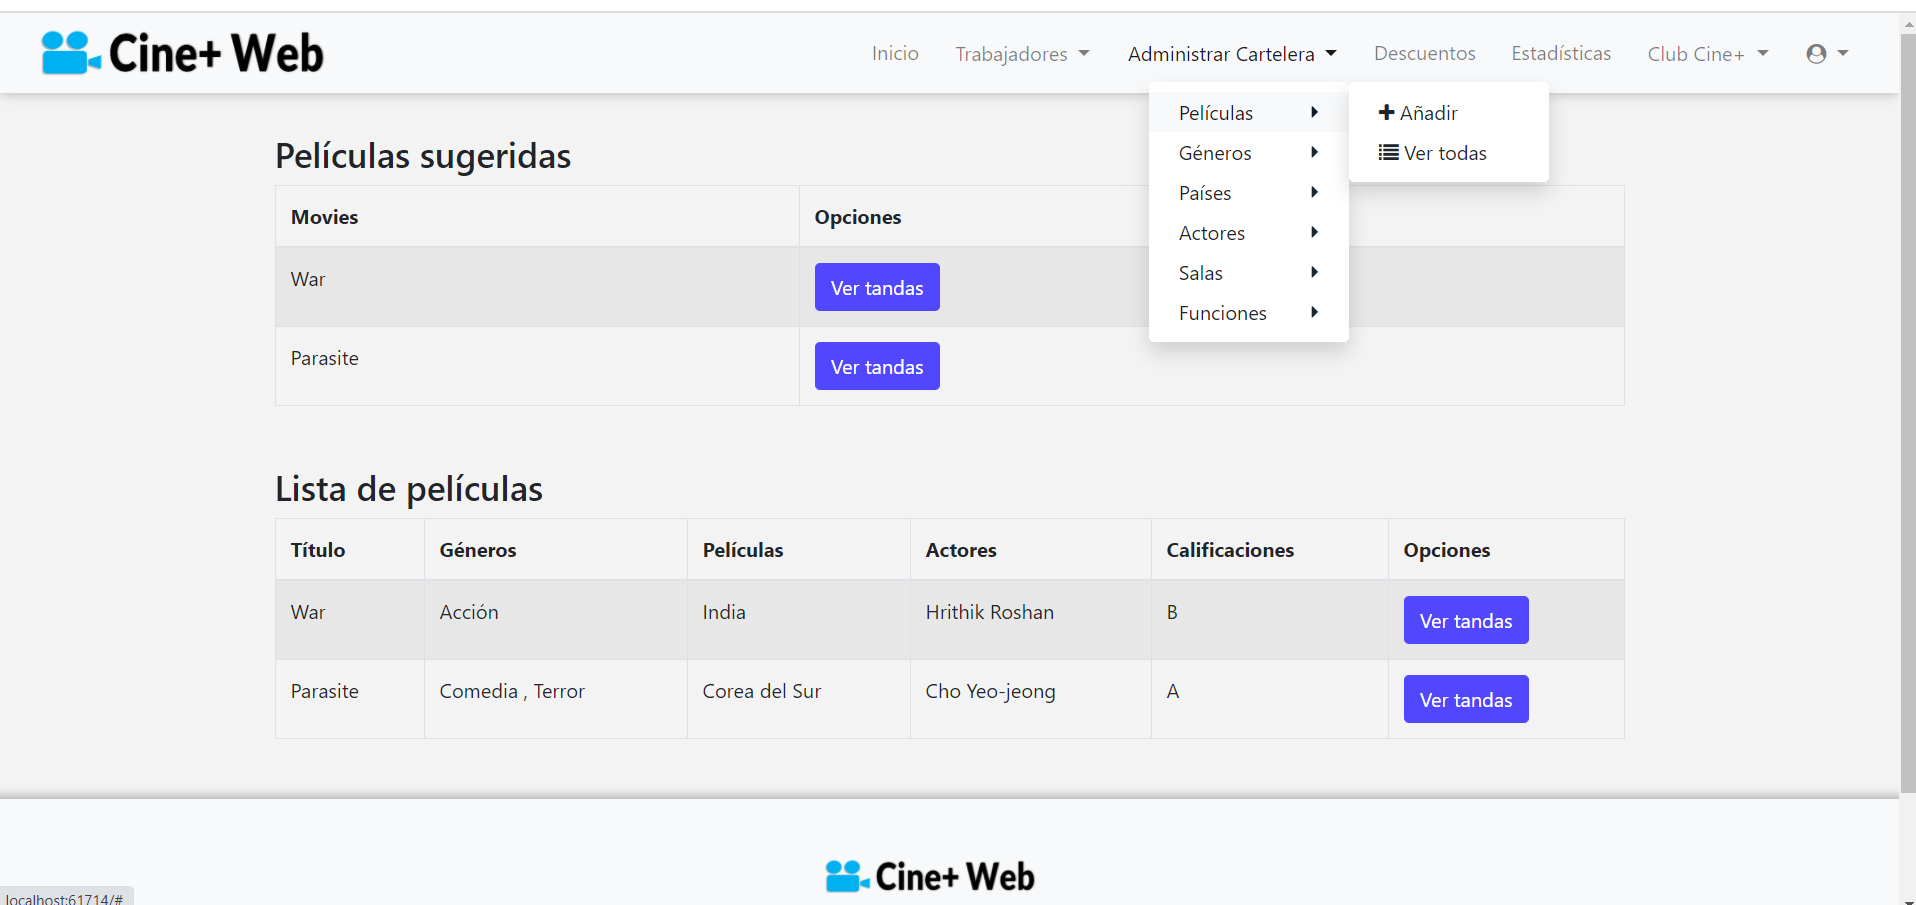
\includegraphics[scale=0.35]{./chapters/img/movie_option.png}
	
	\label{fig:movie_option}
	\caption{Opciones Gestor Pel\'icula}
	
\end{figure}
La opci\'on \verb*|Ver| \verb*|Todas| carga la p\'agina Movies donde se muestra la tabla de las pel\'iculas registradas en la base de datos y la botones para agregar o eliminar estas.

\begin{figure}[h!]
	\centering
	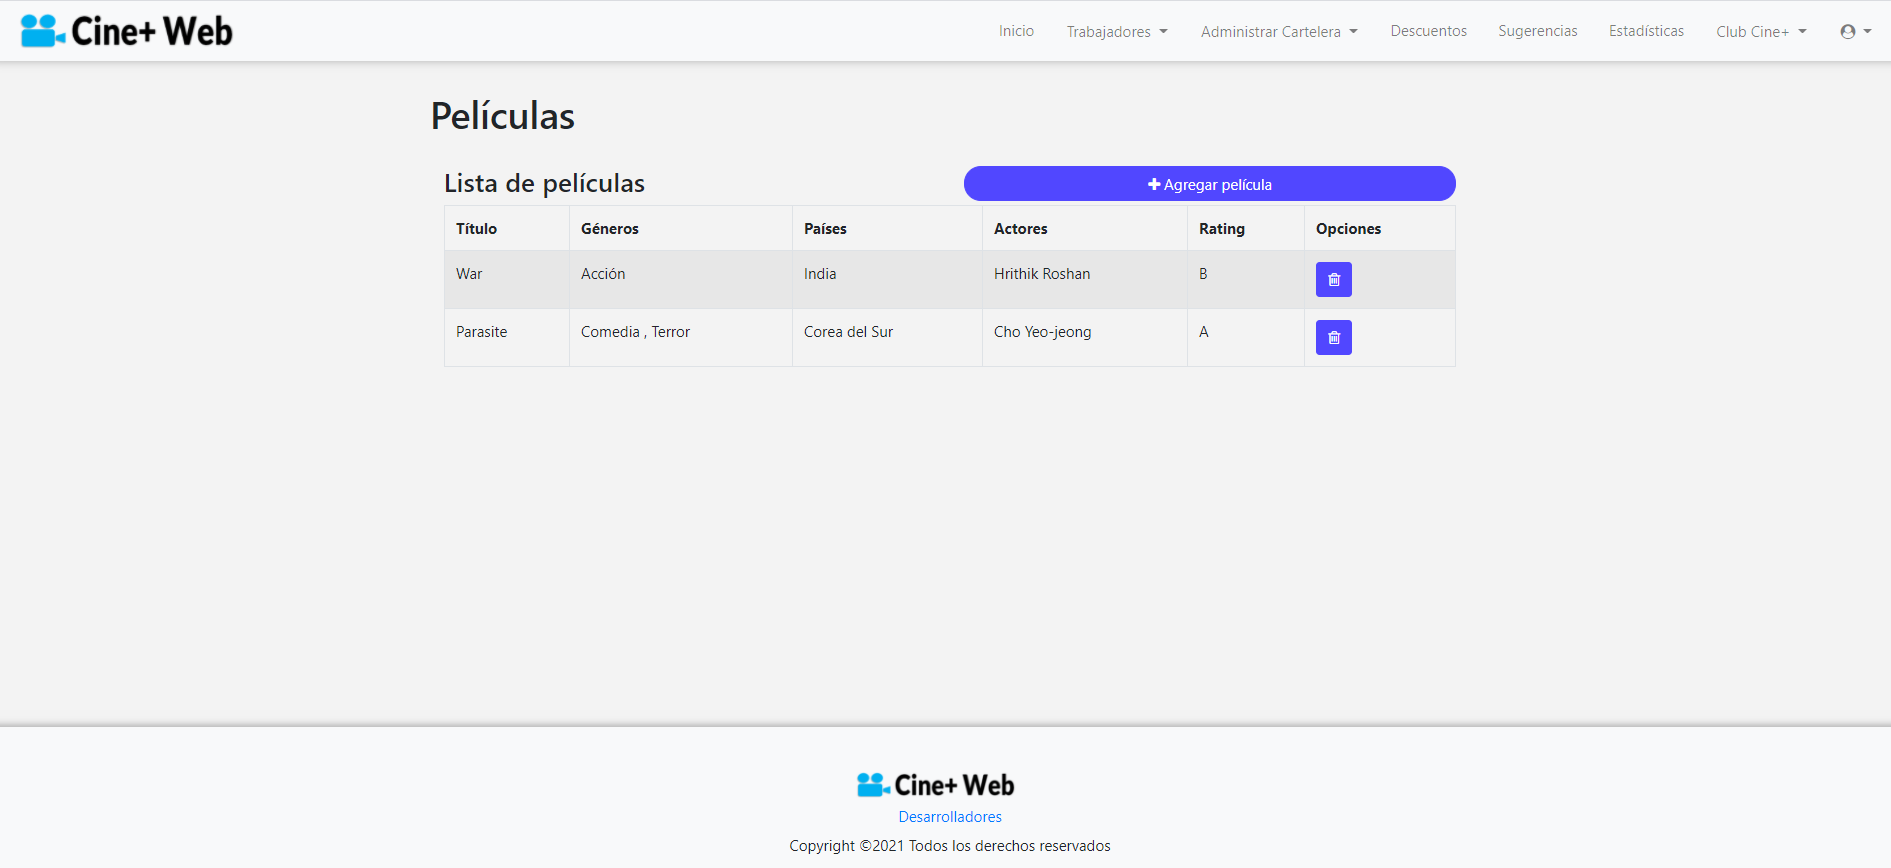
\includegraphics[scale=0.35]{./chapters/img/movies_table.png}
	
	\label{fig:movie_table}
	\caption{P\'agina Movies}
	
\end{figure}

Al agregar una pel\'icula se debe especificar \'el(los) g\'eneros a la que pertenece, la calificaci\'on, pa\'is y los actores que en ella participan as\'i como se observa en la siguiente imagen.
\newpage
\begin{figure}[h!]
	\centering
	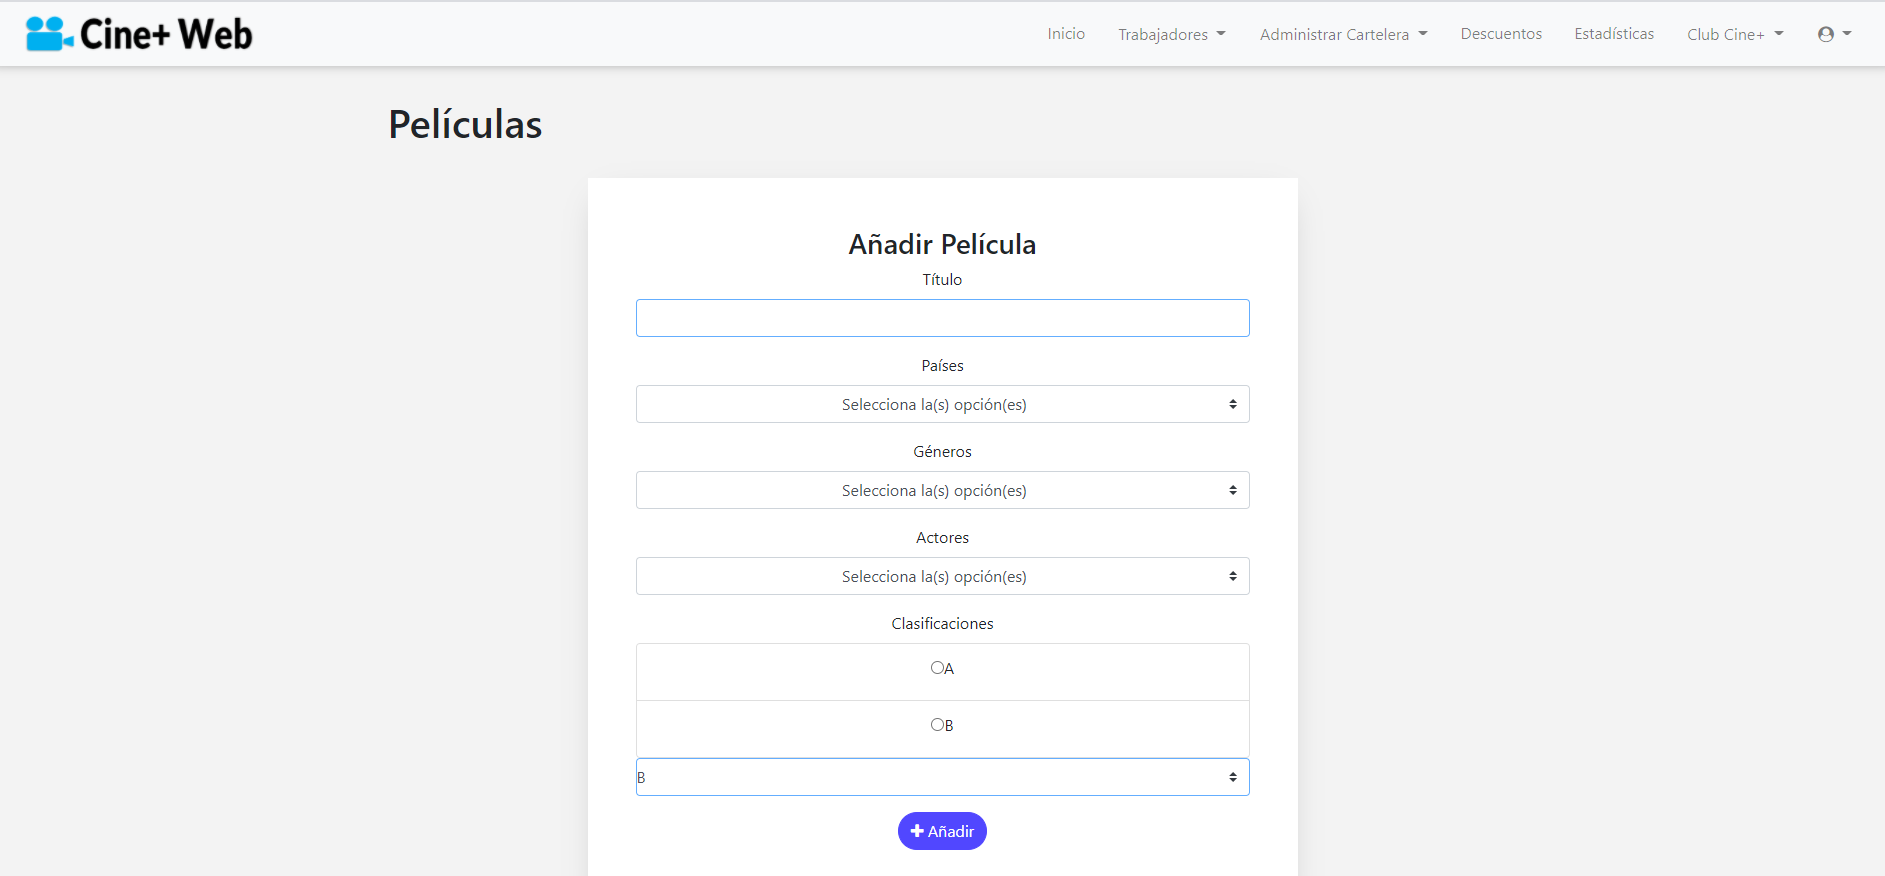
\includegraphics[scale=0.35]{./chapters/img/add_movie.png}
	
	\label{fig:add_movie}
	\caption{Agregar Pel\'icula}
	
\end{figure}

\subsubsection{Gestor de Actores, Pa\'ises, G\'eneros y Salas }

La informaci\'on relacionada con los actores, pa\'ises, g\'eneros y salas se encuentra representada de forma similar que las pel\'iculas. Para la creaci\'on de estos se debe especificar en el caso de g\'enero y pa\'is, el nombre; para los actores, nombre y apellidos y en el otro caso de las salas la capacidad de estas.

\subsubsection{Gestor de Funciones}
La informaci\'on relacionada con las funciones se encuentra representada de forma similar que las pel\'iculas. Para la creaci\'on de estas se debe especificar la fecha de inicio, finalizaci\'on, la sala, la pel\'icula, precio de entrada y precio de la entrada en puntos como se muestra en la siguiente imagen.

\begin{figure}[h!]
	\centering
	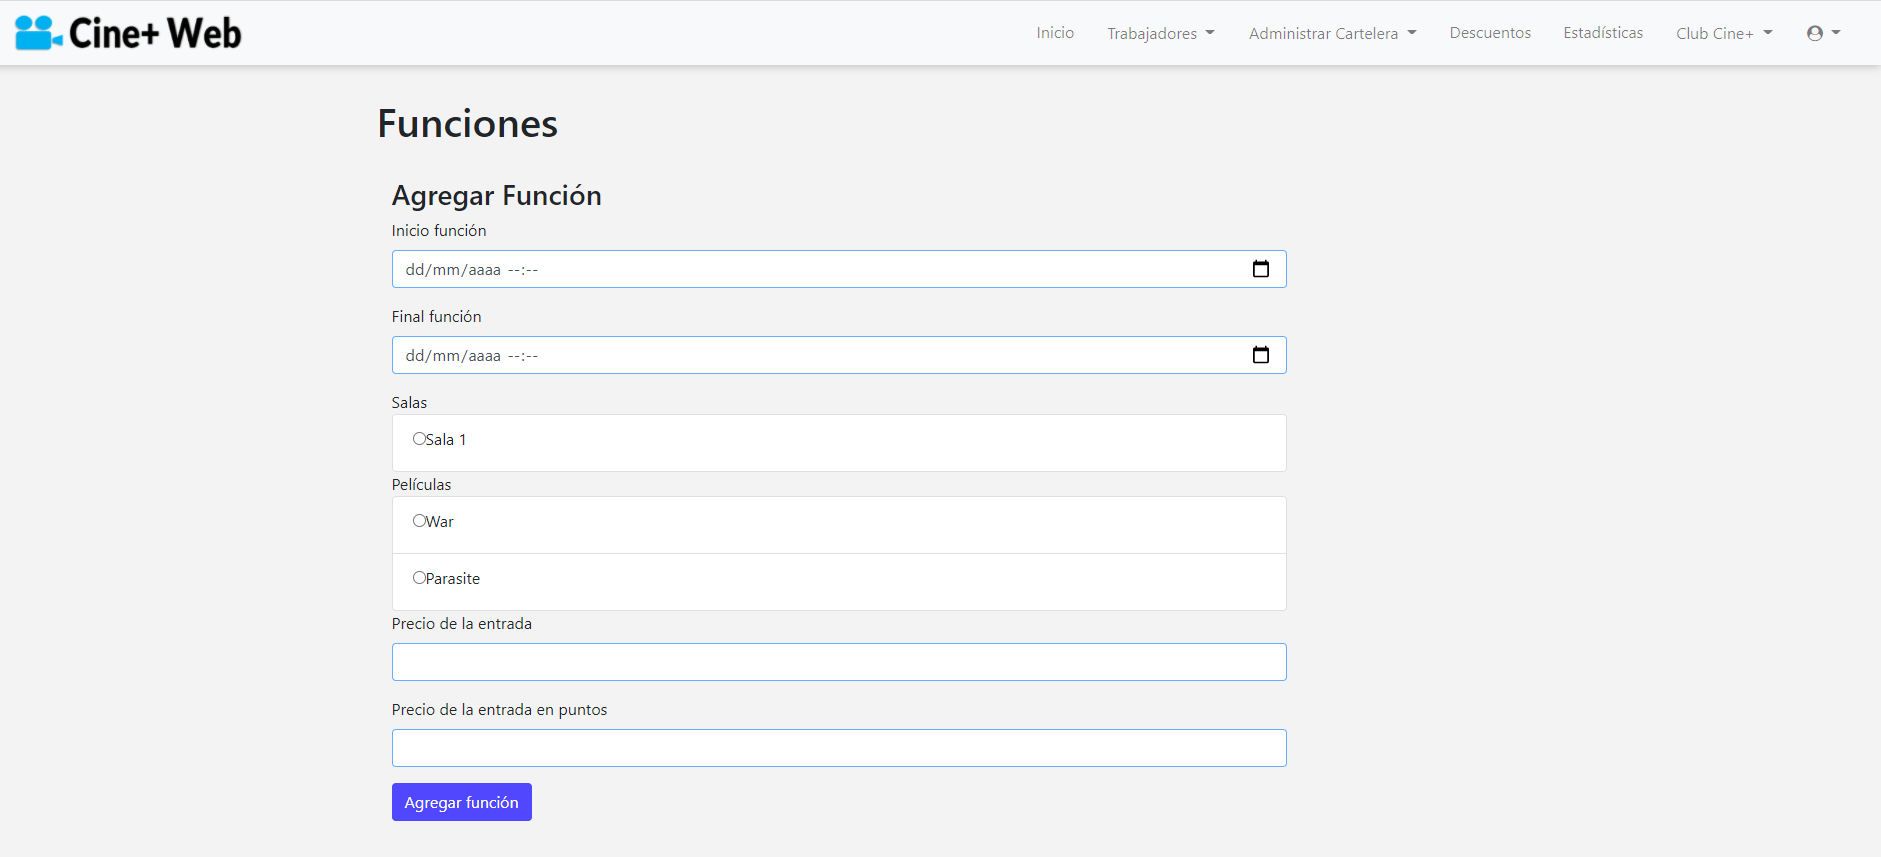
\includegraphics[scale=0.35]{./chapters/img/add_function.png}
	
	\label{fig:add_function}
	\caption{Agregar Funci\'on}
	
\end{figure}

\subsection{Gestor de Socios}
Las opciones referentes a la gesti\'on de socios son accesibles desde la pesta\~na \verb*|Club| \verb*|Cine+| disponible en la cabecera de taquillero y gerente

\begin{figure}[h!]
	\centering
	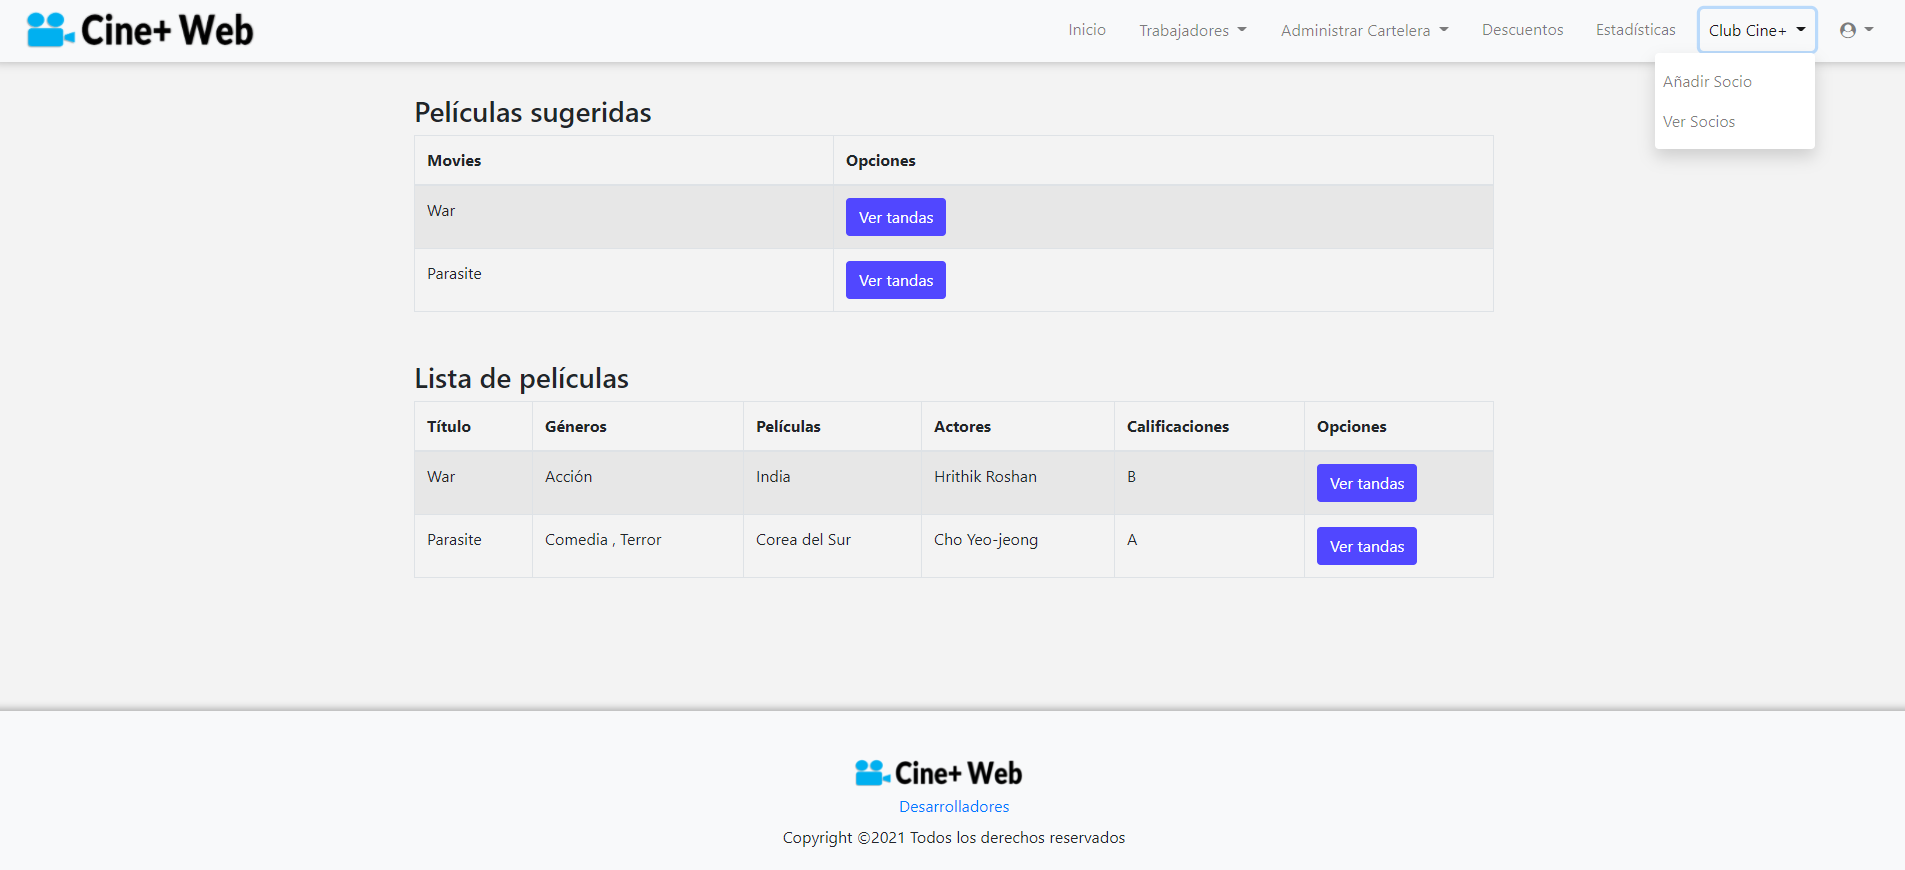
\includegraphics[scale=0.35]{./chapters/img/option_partner.png}
	
	\label{fig:option_partner}
	\caption{Opciones Socios}
	
\end{figure}

La opci\'on \verb*|Ver| \verb*|Socios| direcciona a una p\'agina donde se visualiza el listado de socios registrados y la informaci\'on asociada a estos. De igual manera la opci\'on \verb*|Agregar| \verb*|Socio| permite que los gerentes y taquilleros del cine pueden registrar los socios especificando la informaci\'on asociada a estos en los campos en la p\'agina a la que direcciona como se muestra en la siguiente imagen.

\begin{figure}[h!]
	\centering
	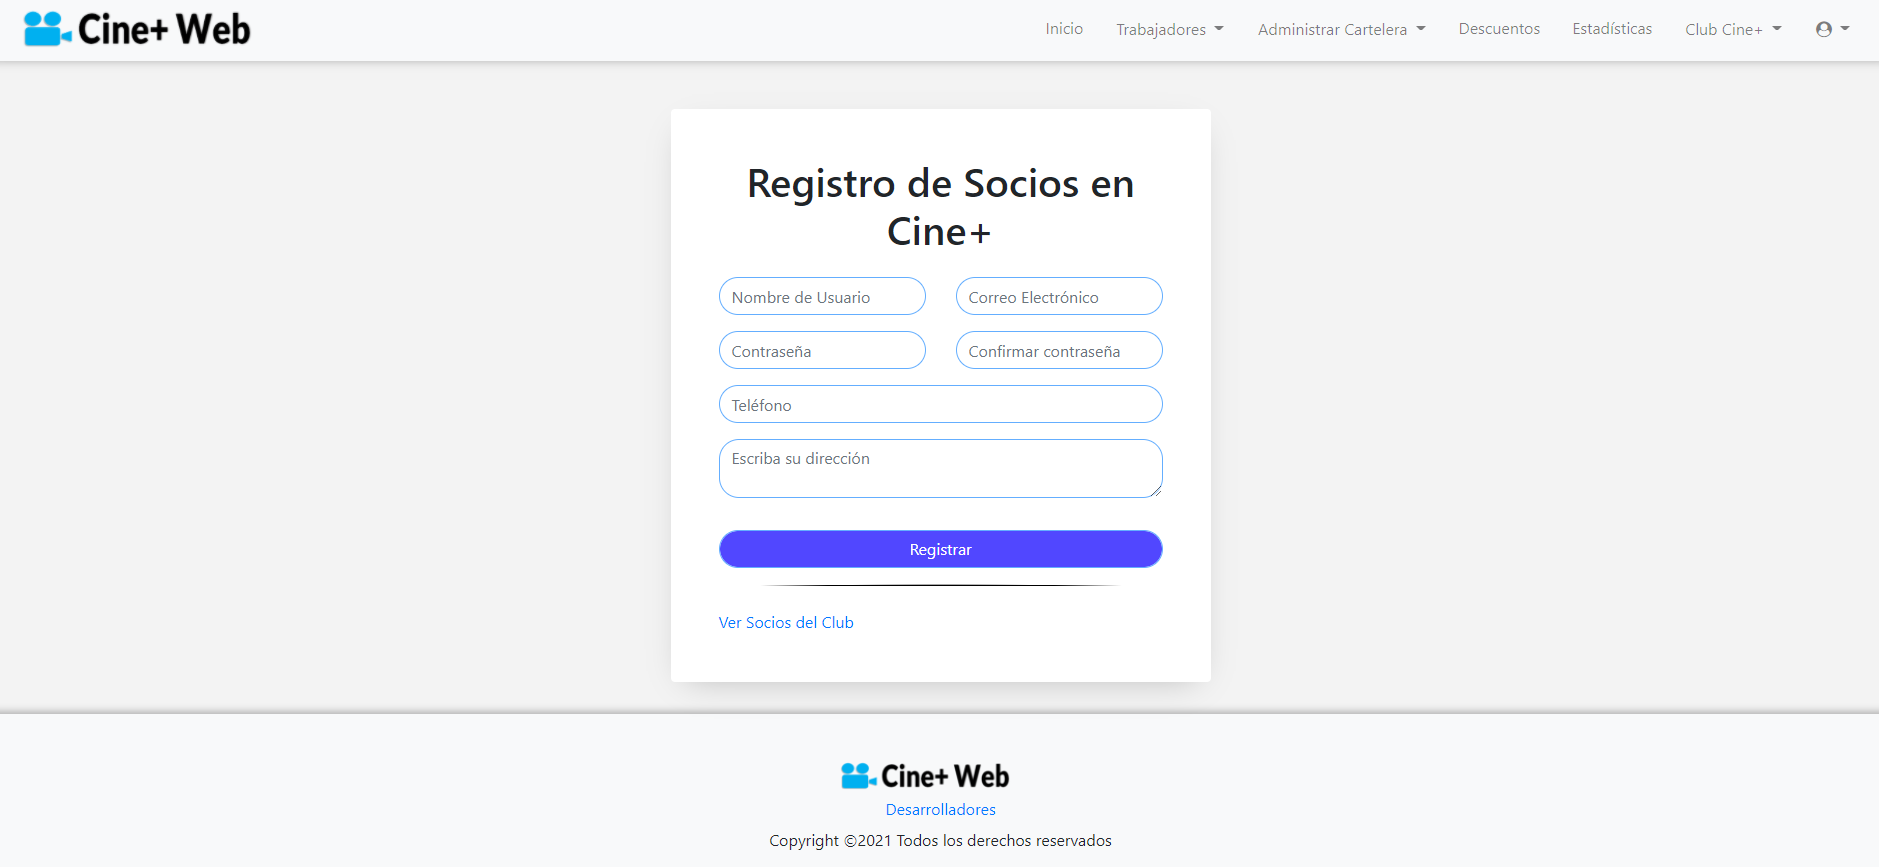
\includegraphics[scale=0.35]{./chapters/img/add_partner.png}
	
	\label{fig:add_partner}
	\caption{Agregar Socio}
	
\end{figure}

\subsection{Gestor de Descuentos}
La pesta\~na \verb*|Descuentos| disponible en la cabecera direcciona a la p\'agina donde se visualiza la lista de descuentos registradas; estas pueden ser editadas o eliminadas. El bot\'on \verb*|Agregar| \verb*|Descuento| redirecciona a la p\'agina donde los gerentes crean estos descuentos especificando los campos nombre y la cantidad de dinero descontado como se muestra en la siguiente imagen.

\begin{figure}[h!]
	\centering
	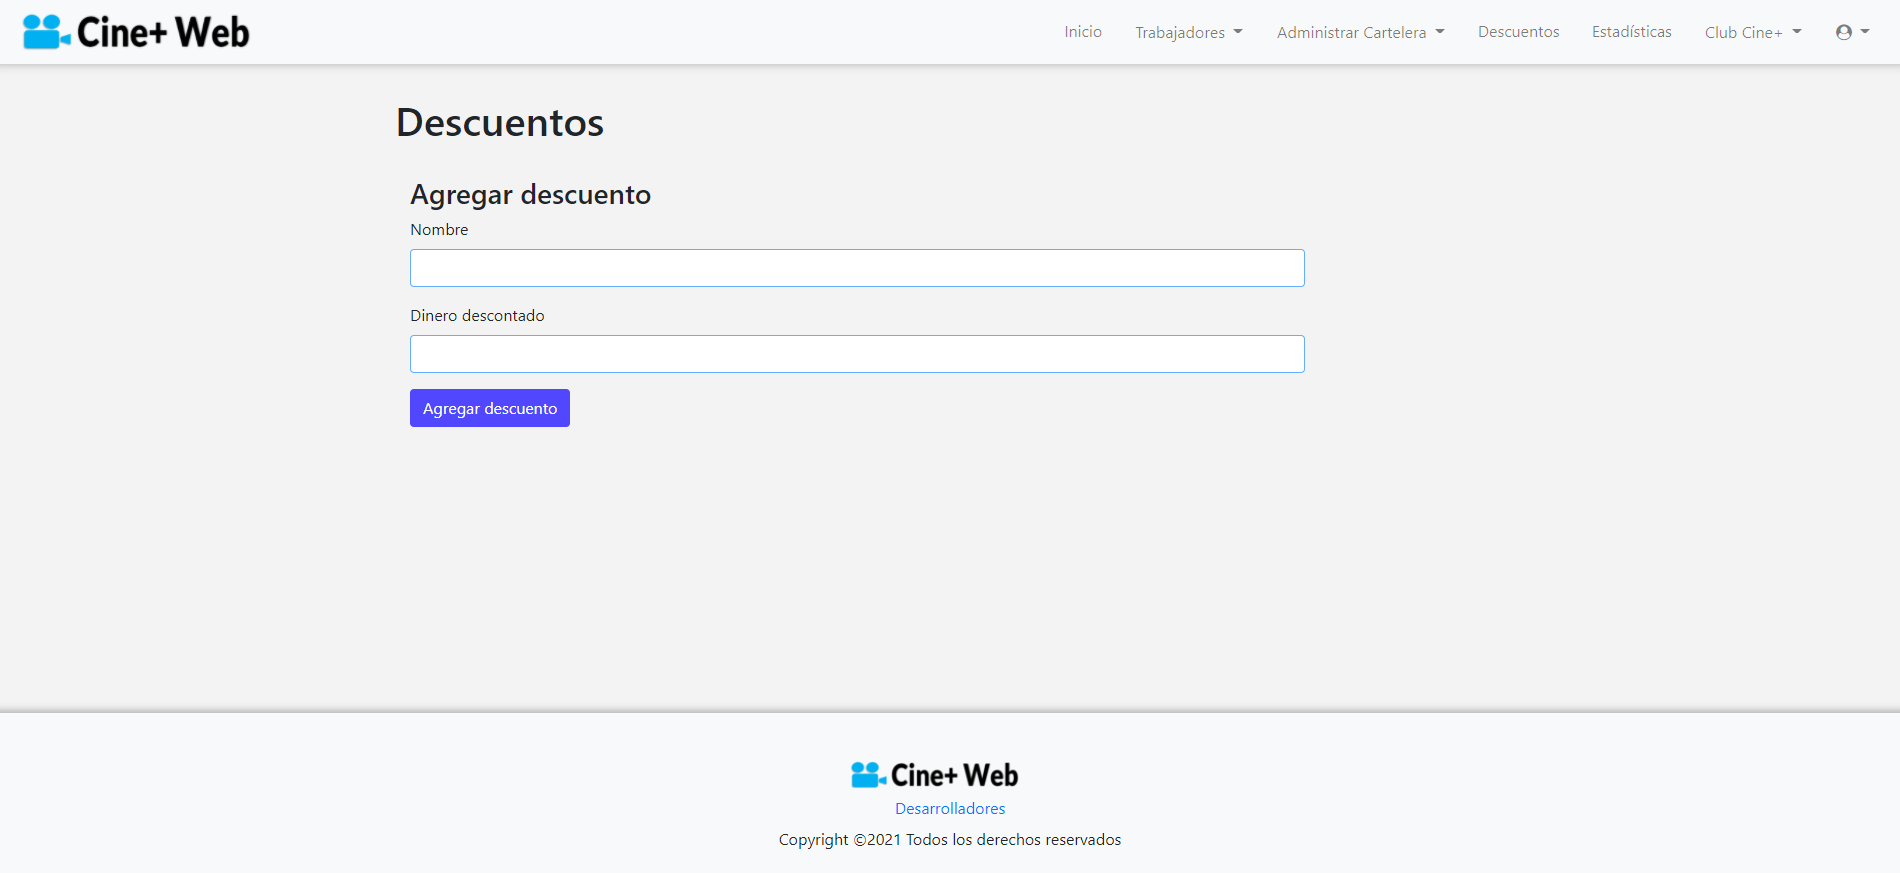
\includegraphics[scale=0.35]{./chapters/img/add_discount.png}
	
	\label{fig:add_discount}
	\caption{Agregar Descuento}
	
\end{figure}



\subsection{Gestor de Trabajadores}
La pesta\~na \verb*|Trabajadores| disponible desde la cabecera de los gerentes despliega dos opciones, la primera \verb*|Taquilleros| la cual direcciona a una p\'agina donde se muestran la informaci\'on referente a los taquilleros registrados y muestra la opci\'on \verb*|Registrar|  \verb*|Taquillero| con un formulario similar al del registro de usuario.

\begin{figure}[h!]
	\centering
	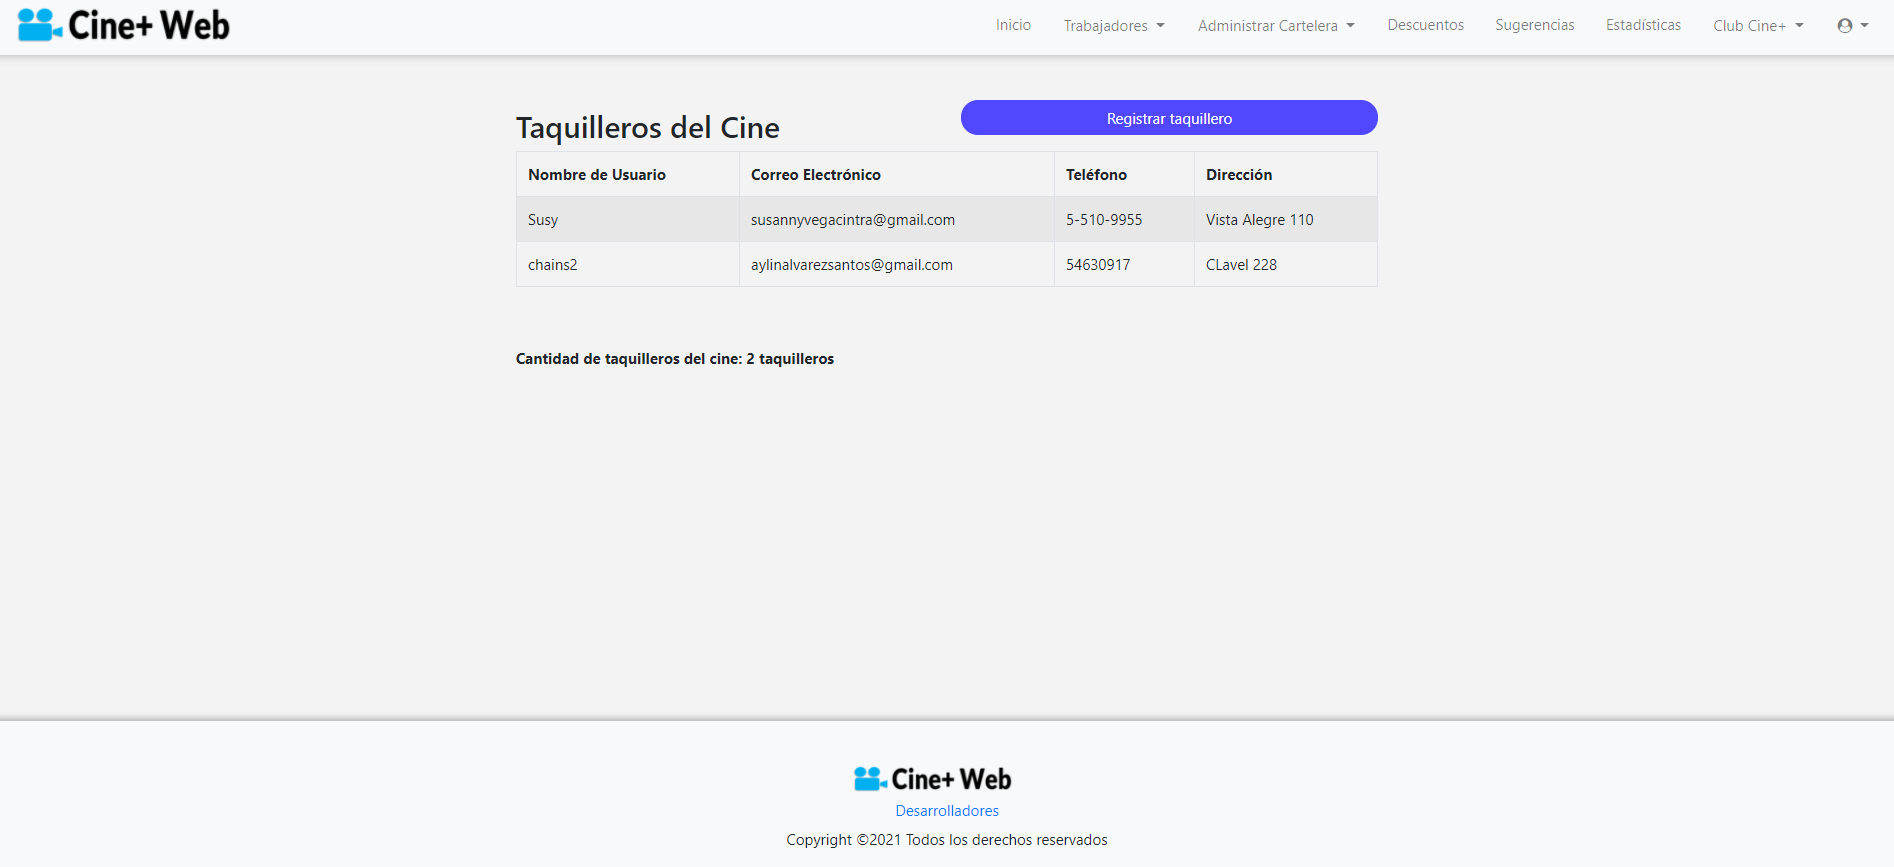
\includegraphics[scale=0.35]{./chapters/img/ver_taquilleros.png}
	
	\label{fig:ver_taquilleros}
	\caption{Taquilleros}
	
\end{figure}

La segunda opci\'on \verb*|Gerentes| direcciona a una p\'agina donde se muestran la informaci\'on referente a los gerentes registrados y muestra la opci\'on \verb*|Registrar|  \verb*|Gerente| con un formulario similar al del registro de usuario.
\newpage
\begin{figure}[h!]
	\centering
	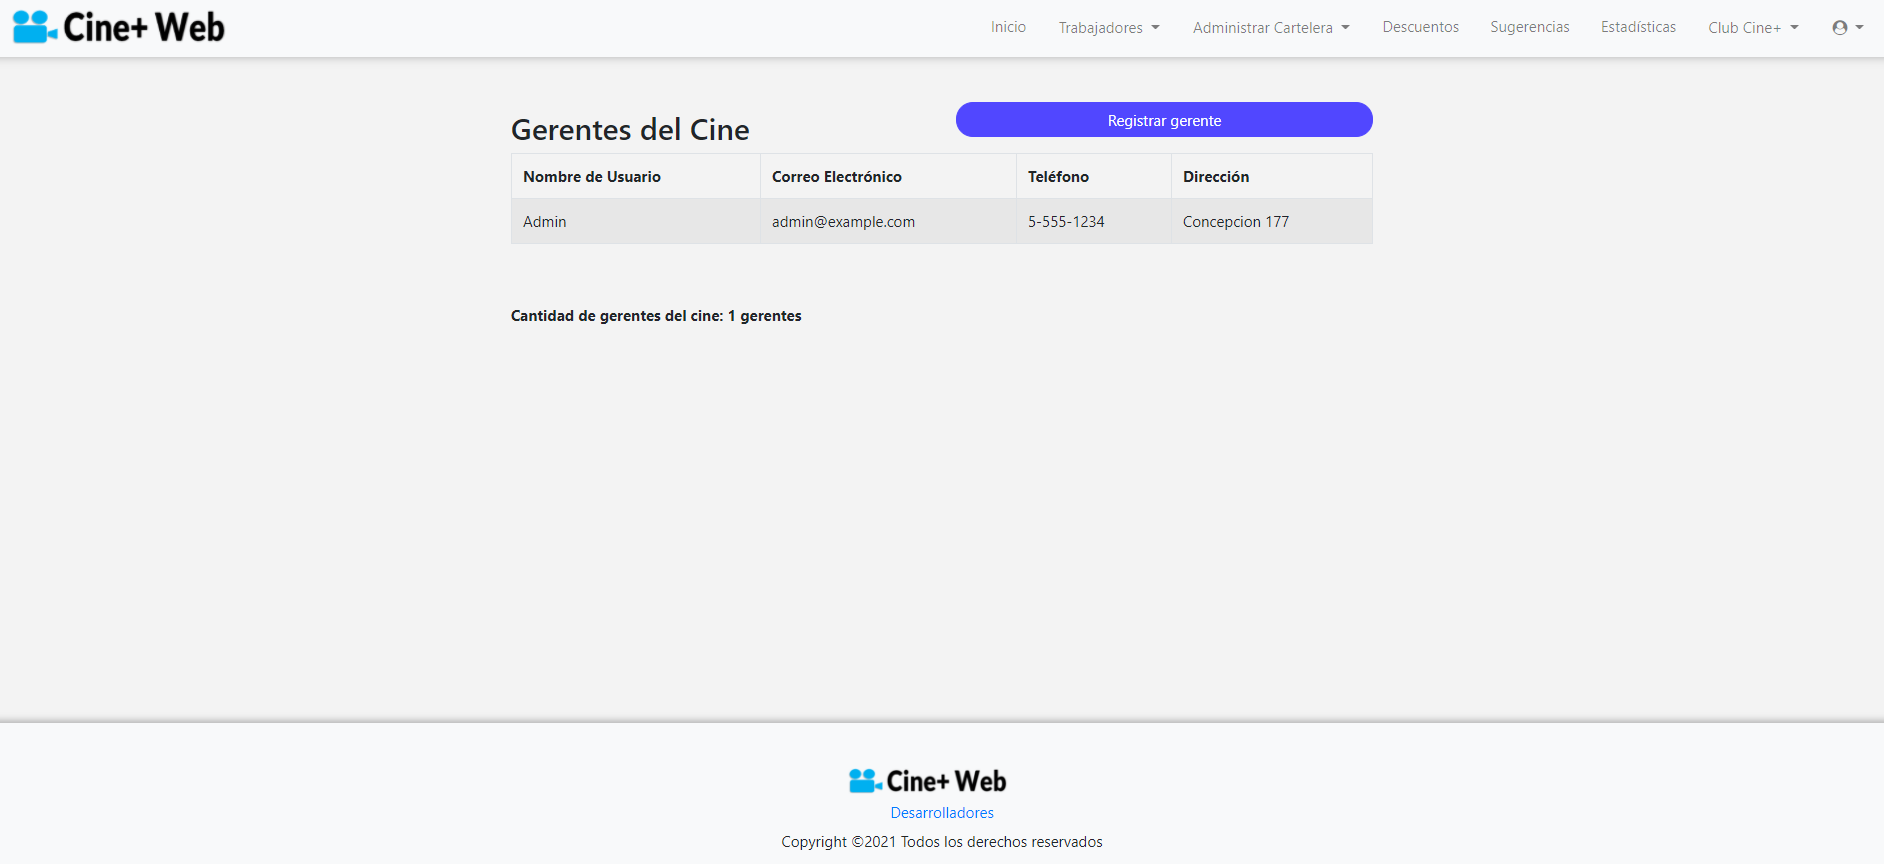
\includegraphics[scale=0.35]{./chapters/img/ver_gerentes.png}
	
	\label{fig:ver_gerentes}
	\caption{Gerentes}
	
\end{figure}

\subsection{Sugerencias}
Esta opci\'on es accesible desde las cabecera de los gerentes, esta direcciona a una p\'agina donde se muestran los criterios a aplicar en la sugerencia de pel\'iculas que se muestra en la p\'agina inicial de la aplicaci\'on.

\begin{figure}[h!]
	\centering
	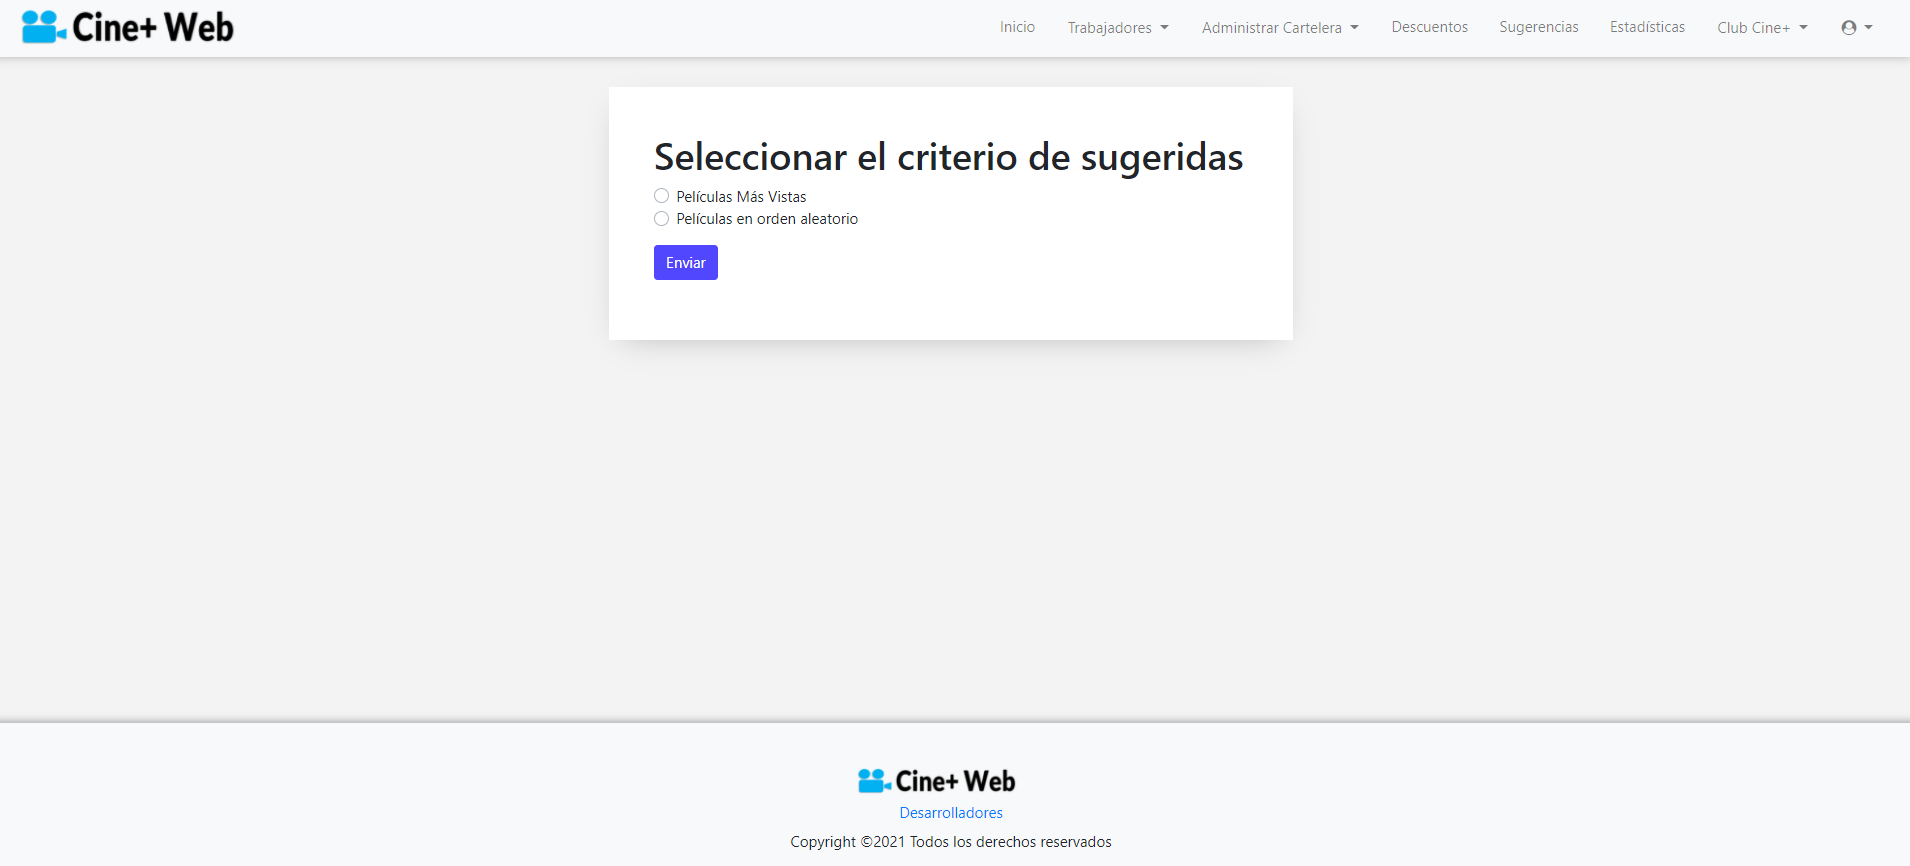
\includegraphics[scale=0.35]{./chapters/img/criteria.png}
	
	\label{fig:criteria}
	\caption{Sugerencias}
	
\end{figure}

\subsection{Estad\'isticas}
Esta opci\'on es accesible desde las cabecera de los gerentes, esta direcciona a una p\'agina donde se muestran las diferentes opciones para la consulta de ventas seg\'un el filtro escogido.
\newpage
\begin{figure}[h!]
	\centering
	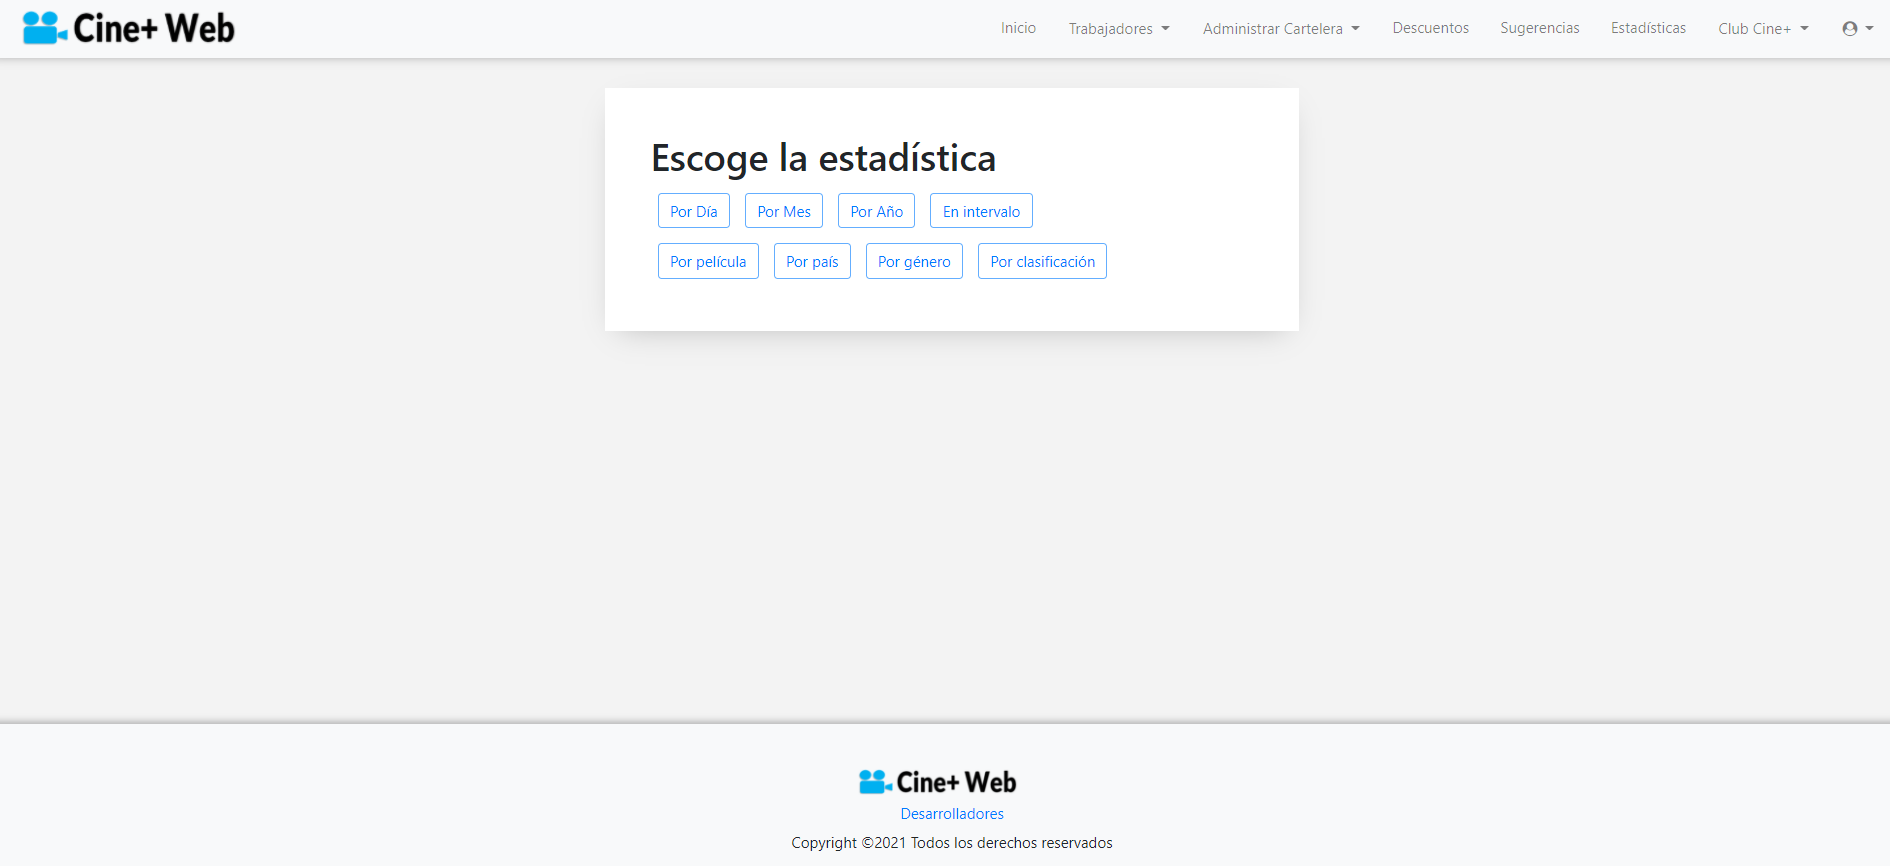
\includegraphics[scale=0.35]{./chapters/img/statistics.png}
	
	\label{fig:statistics}
	\caption{Estad\'isticas}
	
\end{figure}
\subsection{Compra de entradas}
Un usuario logueado o no, puede visualizar las funciones tanto desde la p\'agina inicial accediendo a las tandas desde el bot\'on ubicado en el mismo rengl\'on de la pel\'icula referida como desde la pesta\~na Cartelera disponible en la cabecera para los usuarios clientes, esta \'ultima al hacer click direcciona a la p\'agina donde se muestra el listado de funciones, en cada rengl\'on se muestra una funci\'on y las opciones asociadas a estas.\\

\subsubsection{Paso 1}
En este paso se muestra el campo de C\'odigo de Socio que puede ser especificado en caso del  estar registrado como socio y en el campo el N\'umero de entradas se debe especificar la cantidad de estas, para avanzar se debe hacer click en el bot\'on \verb*|Aceptar|\\

\begin{figure}[h!]
	\centering
	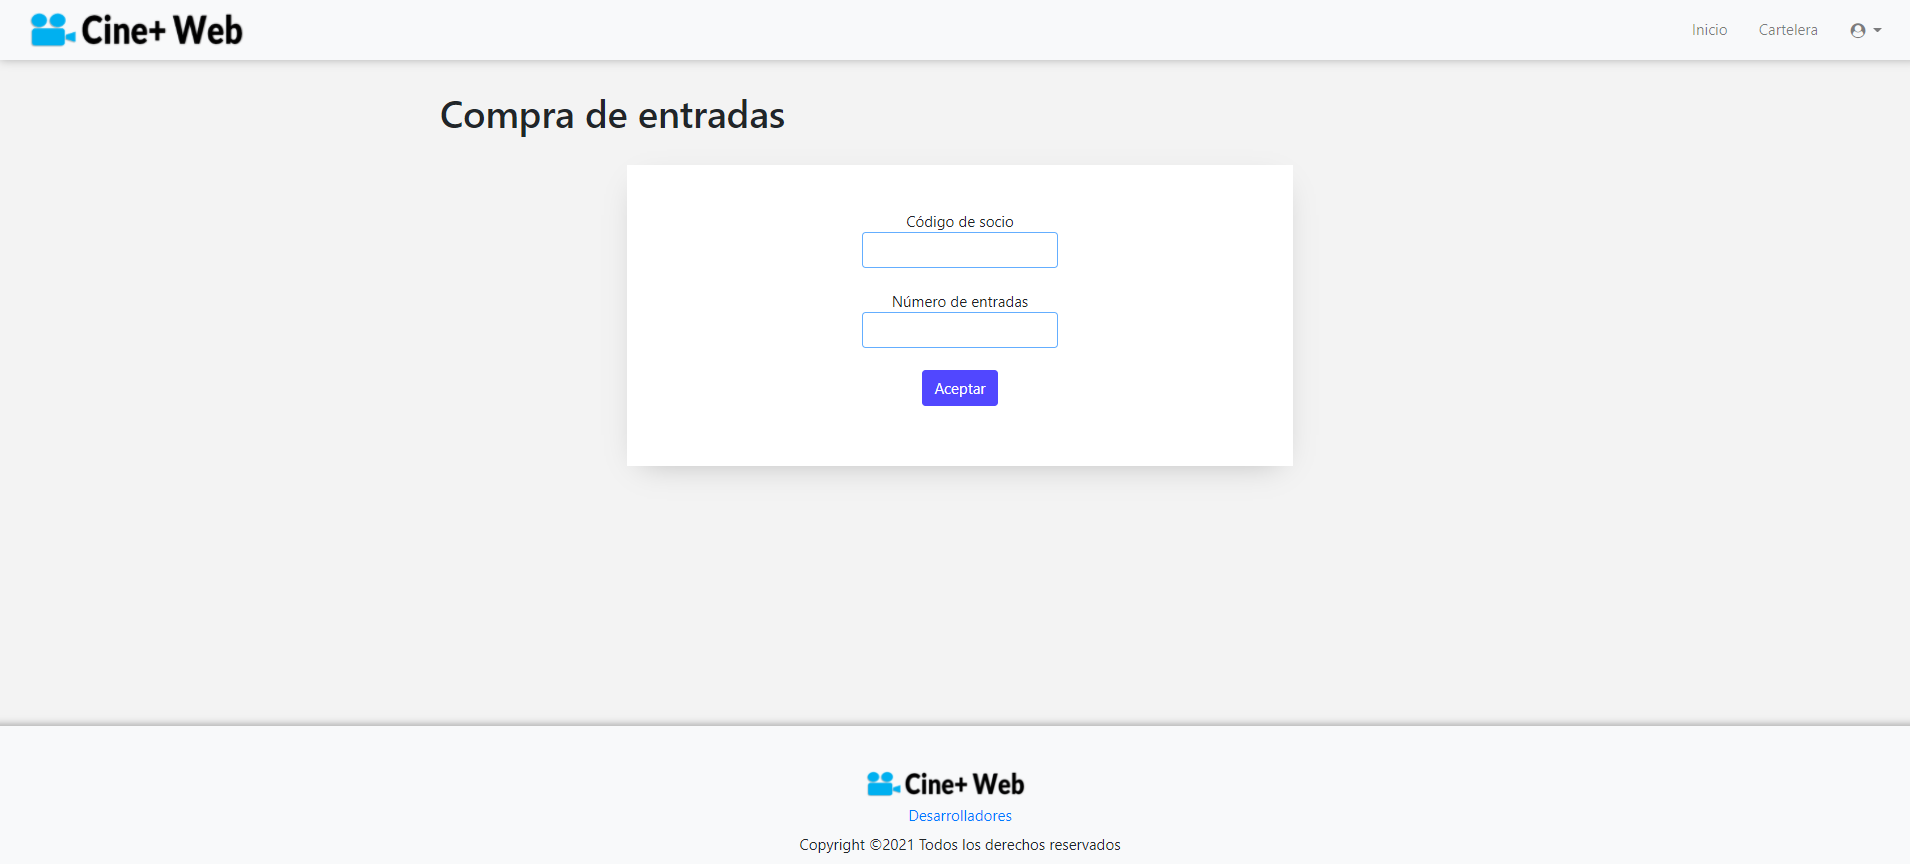
\includegraphics[scale=0.35]{./chapters/img/ticketpurchase1.png}
	
	\label{fig:ticketpurchase1}
	\caption{Compra de entradas}
	
\end{figure}

\subsubsection{Paso 2}
En este paso se muestra las sillas disponibles de la sala donde se puede seleccionar a conveniencia, el sistema autom\'aticamente seleccionar\'a de forma consecutiva en caso de estar disponibles de acuerdo a la cantidad especificada en el paso anterior, para avanzar se debe hacer click en el bot\'on \verb*|Enviar| \verb*|Sillas|.

\begin{figure}[h!]
	\centering
	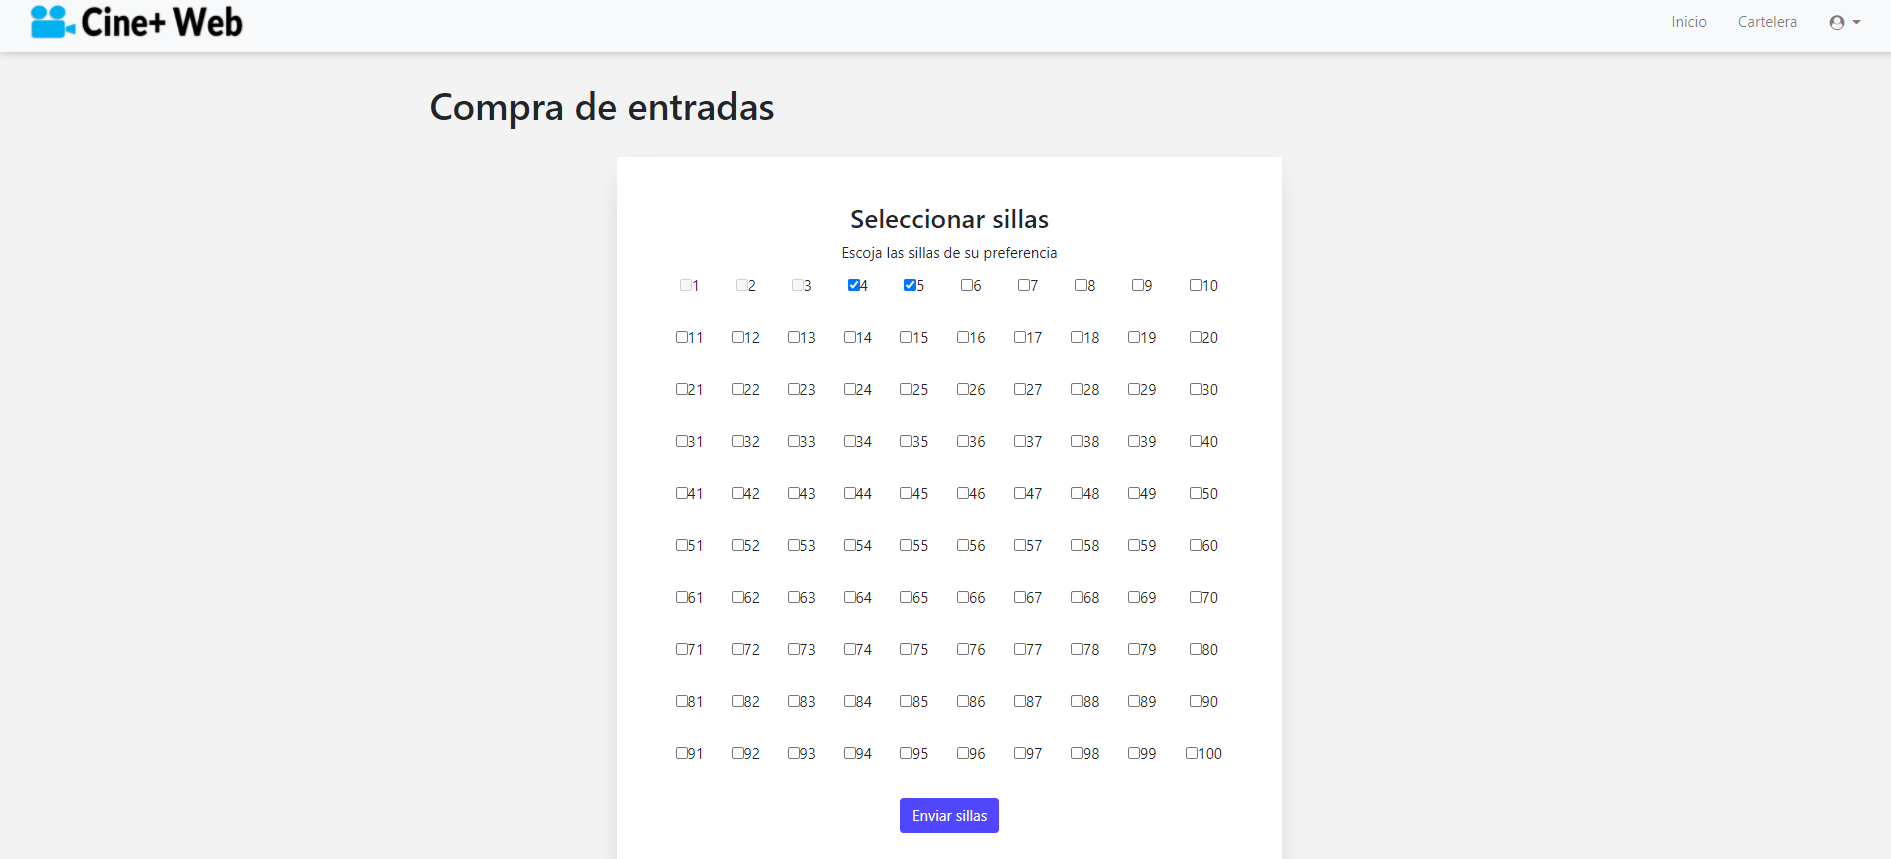
\includegraphics[scale=0.35]{./chapters/img/seat.png}
	
	\label{fig:seats}
	\caption{Seleccionar Sillas}
\end{figure}

\subsubsection{Paso 3}
En este paso se muestra la lista de descuentos disponibles a aplicar para cada silla. En caso que se desee puede especificar por cada silla el descuento a aplicar, luego debe proceder a reservar las silla ya sea la cantidad especificada inicial o una cantidad menor a esta, para avanzar se debe hacer click en el bot\'on \verb*|Pagar|.

\begin{figure}[h!]
	\centering
	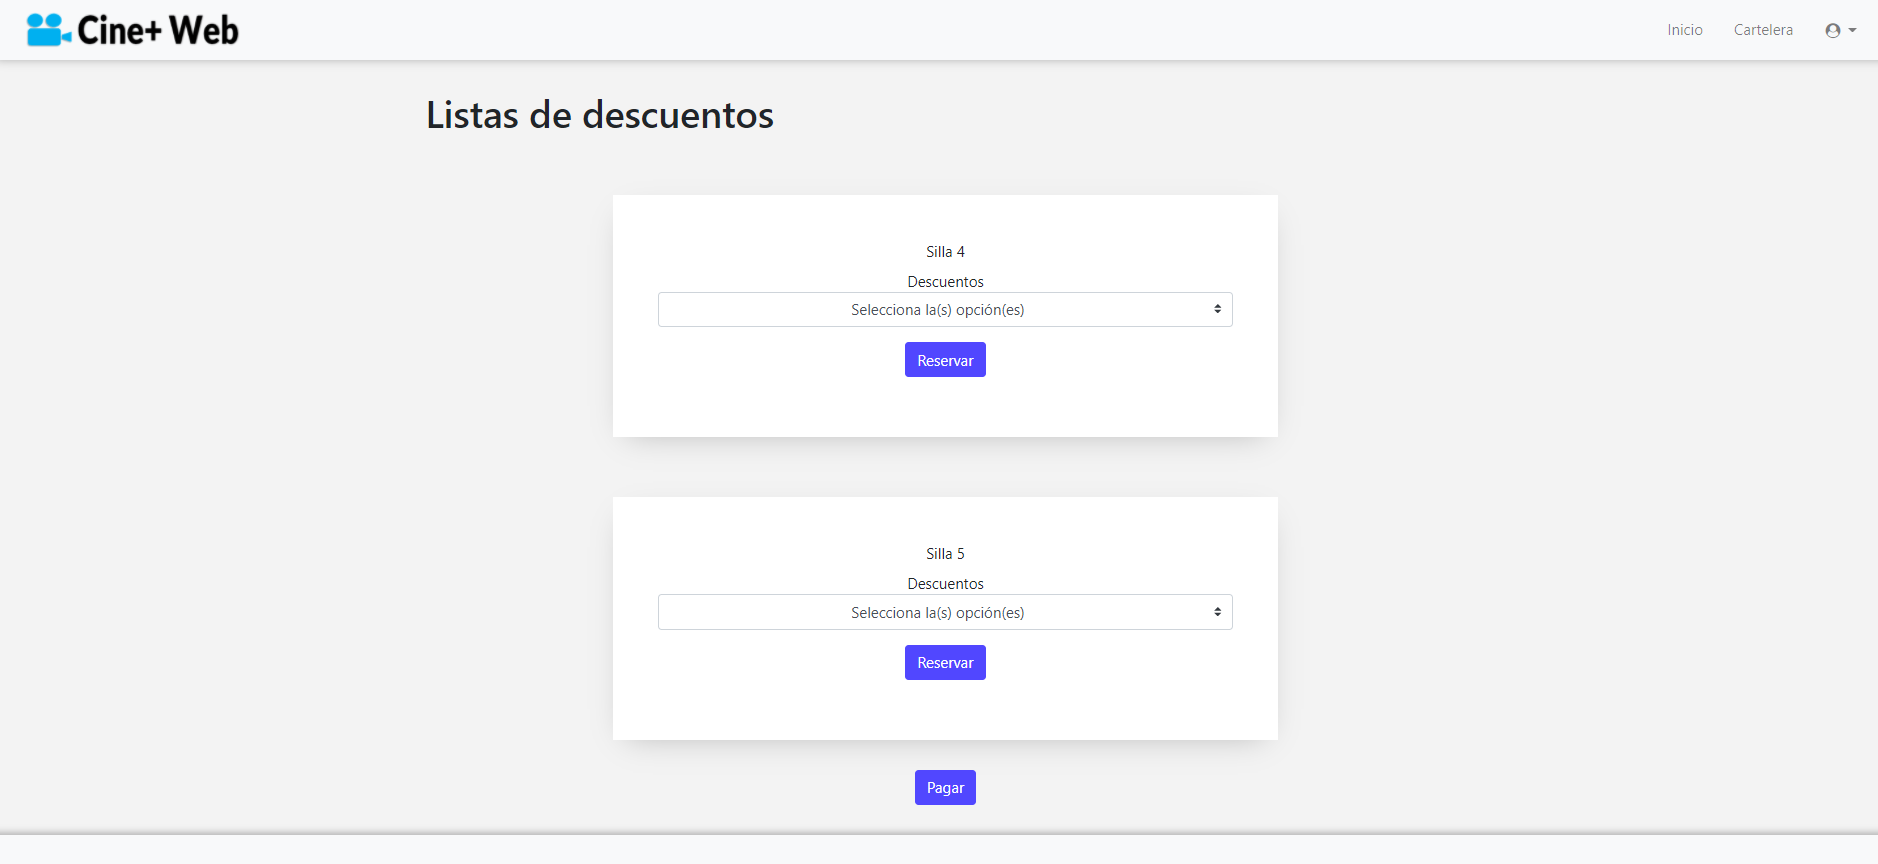
\includegraphics[scale=0.35]{./chapters/img/reserve.png}
	
	\label{fig:reserve}
	\caption{Reservar Sillas}
\end{figure}

\subsubsection{Paso 4}
En este paso se muestra el total a pagar con dinero y con puntos, este \'ultimo aparece en caso de que sea especificado el c\'odigo de socio en el paso 1. Adem\'as aparecen el campo tarjeta de cr\'edito y la opci\'on de pagar con dinero. En caso que se desee pagar con dinero se deber\'a especificar el n\'umero de tarjeta de cr\'edito solo en compras online en el campo correspondiente, en otro caso, se podr\'a pagar con puntos en caso de tener los puntos suficientes para la compra, para esta opci\'on no se debe activar la opci\'on  Pagar con Puntos. Para avanzar al pr\'oximo paso se hacer click en el bot\'on \verb*|Pagar|.

\begin{figure}[h!]
	\centering
	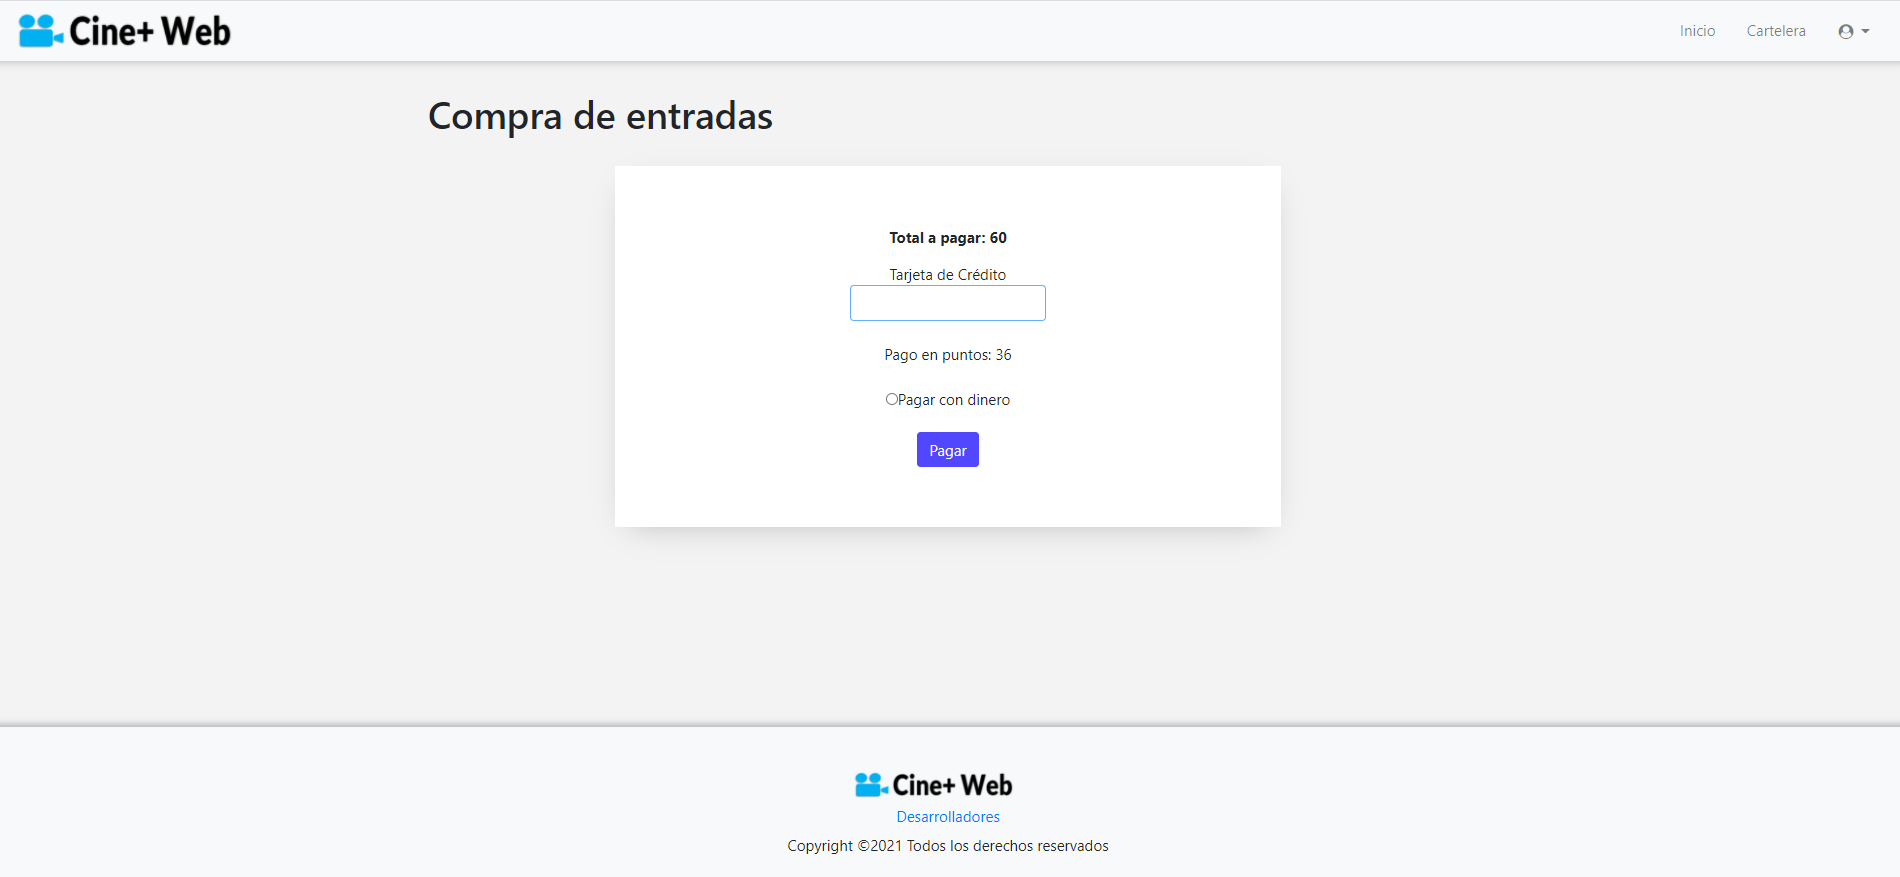
\includegraphics[scale=0.35]{./chapters/img/ticketpurchase2.png}
	
	\label{fig:ticketpurchase2}
	\caption{Tickect de compra}
	
\end{figure}


\subsubsection{Paso 5}
En este paso se muestra el c\'odigo de compra. El cliente debe guardarlo en caso que se desee cancelar la reservaci\'on

\begin{figure}[h!]
	\centering
	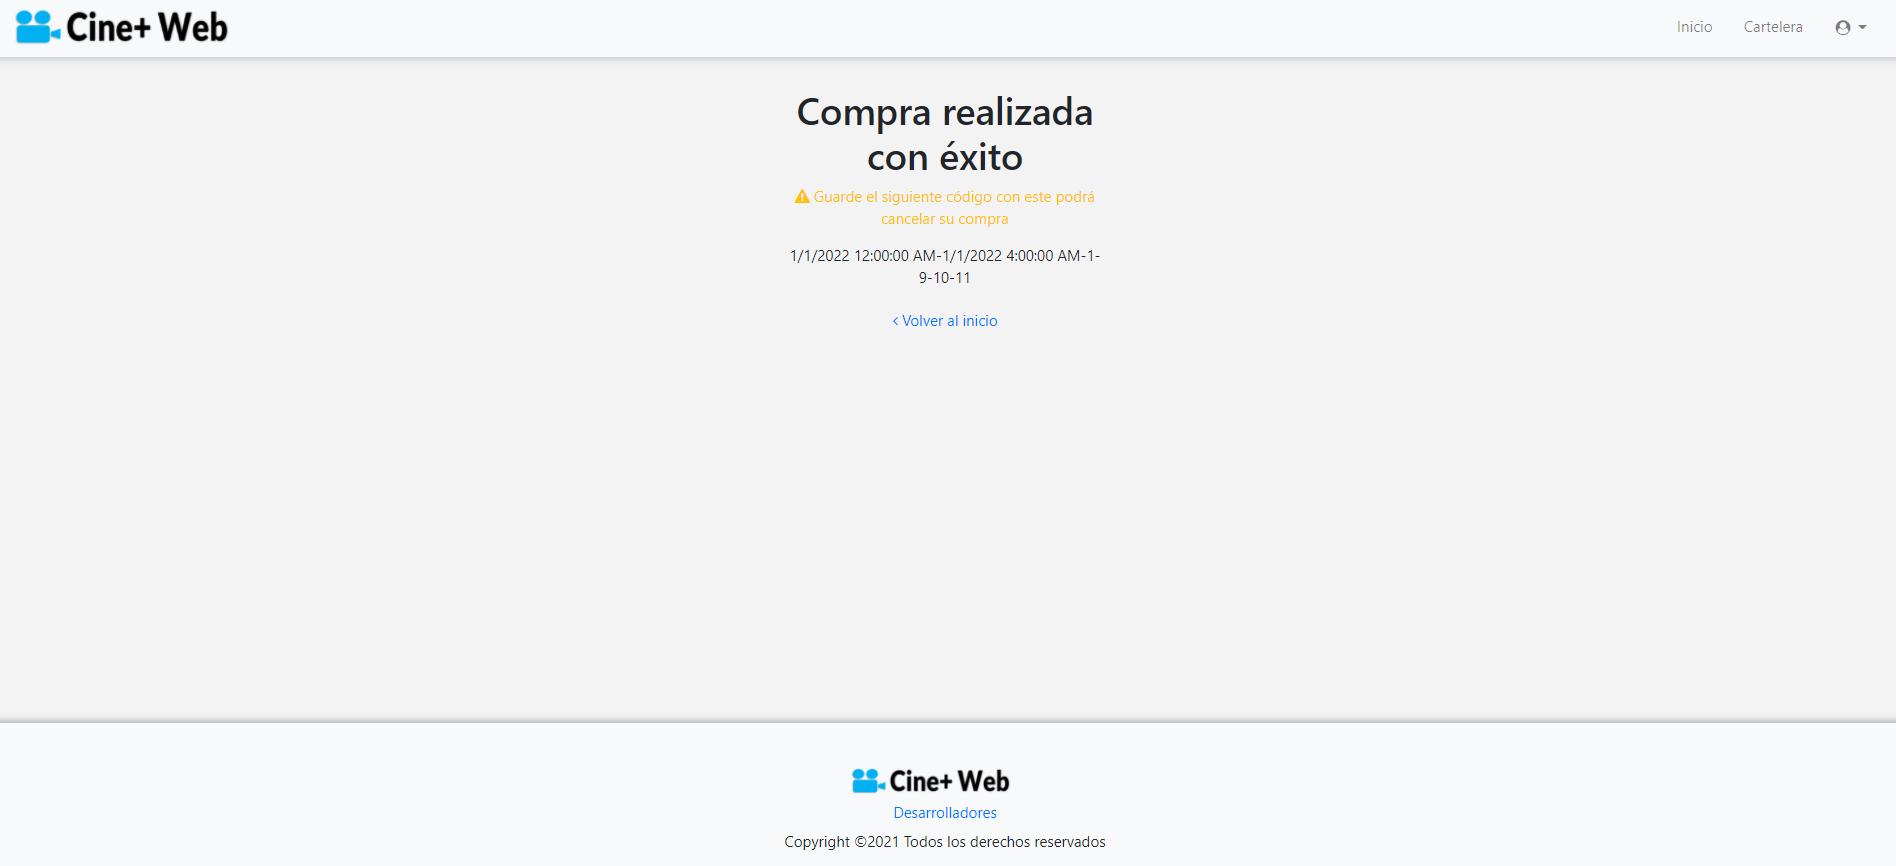
\includegraphics[scale=0.35]{./chapters/img/ticketpurchase3.png}
	
	\label{fig:ticketpurchase3}
	\caption{Tickect de compra}
	
\end{figure}

\subsection{Cancelaci\'on de compras}
Esta opci\'on se muestra junto a la opci\'on de compra en cada regl\'on de funciones, mediante un bot\'on que direcciona a una p\'agina donde se muestra el campo de c\'odigo de socio o tarjeta de cr\'edito y el c\'odigo de compra. EL primero de estos debe ser especificado en el caso de que el pago haya sido realizado por medio de una tarjeta de cr\'edito, especificar esta; o si se realiz\'o por los puntos de socio, especificar el c\'odigo del socio, el \'ultimo campo se debe rellenar con el c\'odigo mostrado en el ticket al efectuar la compra

\begin{figure}[h!]
	\centering
	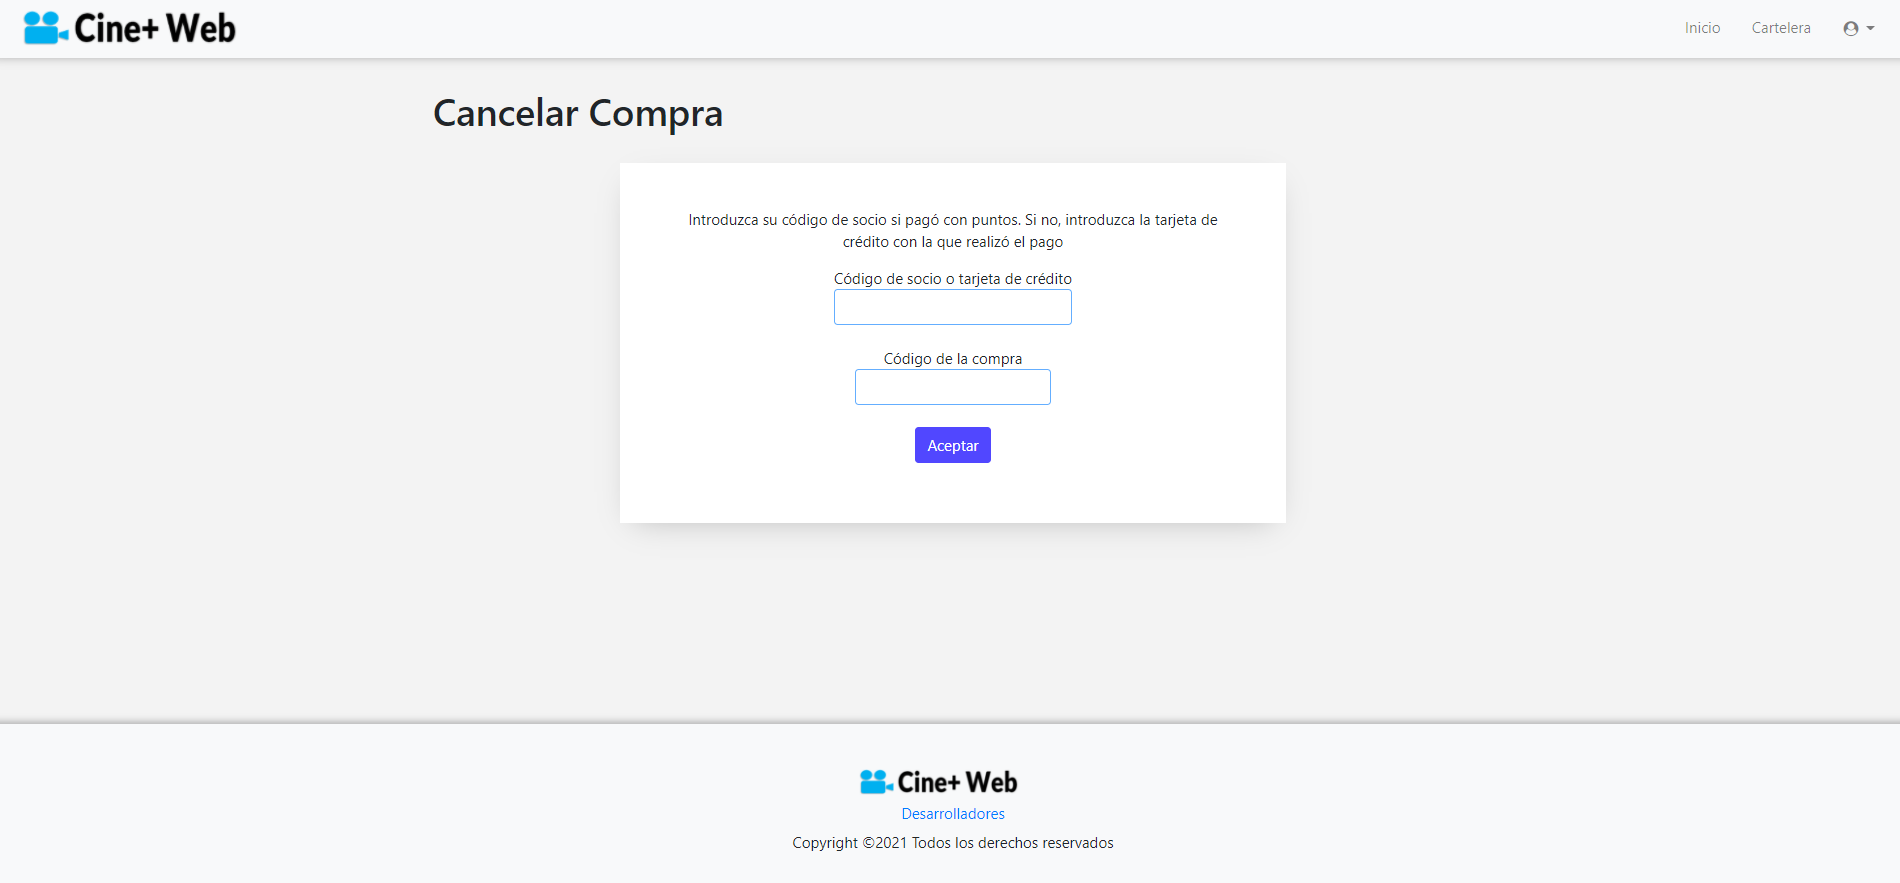
\includegraphics[scale=0.35]{./chapters/img/cancel.png}
	
	\label{fig:cancel}
	\caption{Cancelar compra}
	
\end{figure}
\subsection{Informaci\'on Personal}
El usuario puede visualizar su informaci\'on personal accediendo desde la pesta\~na con el \'icono de usuario, al hacer click en esta aparece la opci\'on Informaci\'on Personal, la que direcciona a una p\'agina donde se muestran los datos introducidos por el usuario en el registro de su cuenta adem\'as del c\'odigo de socio generado por el sistema.

\begin{figure}[h!]
	\centering
	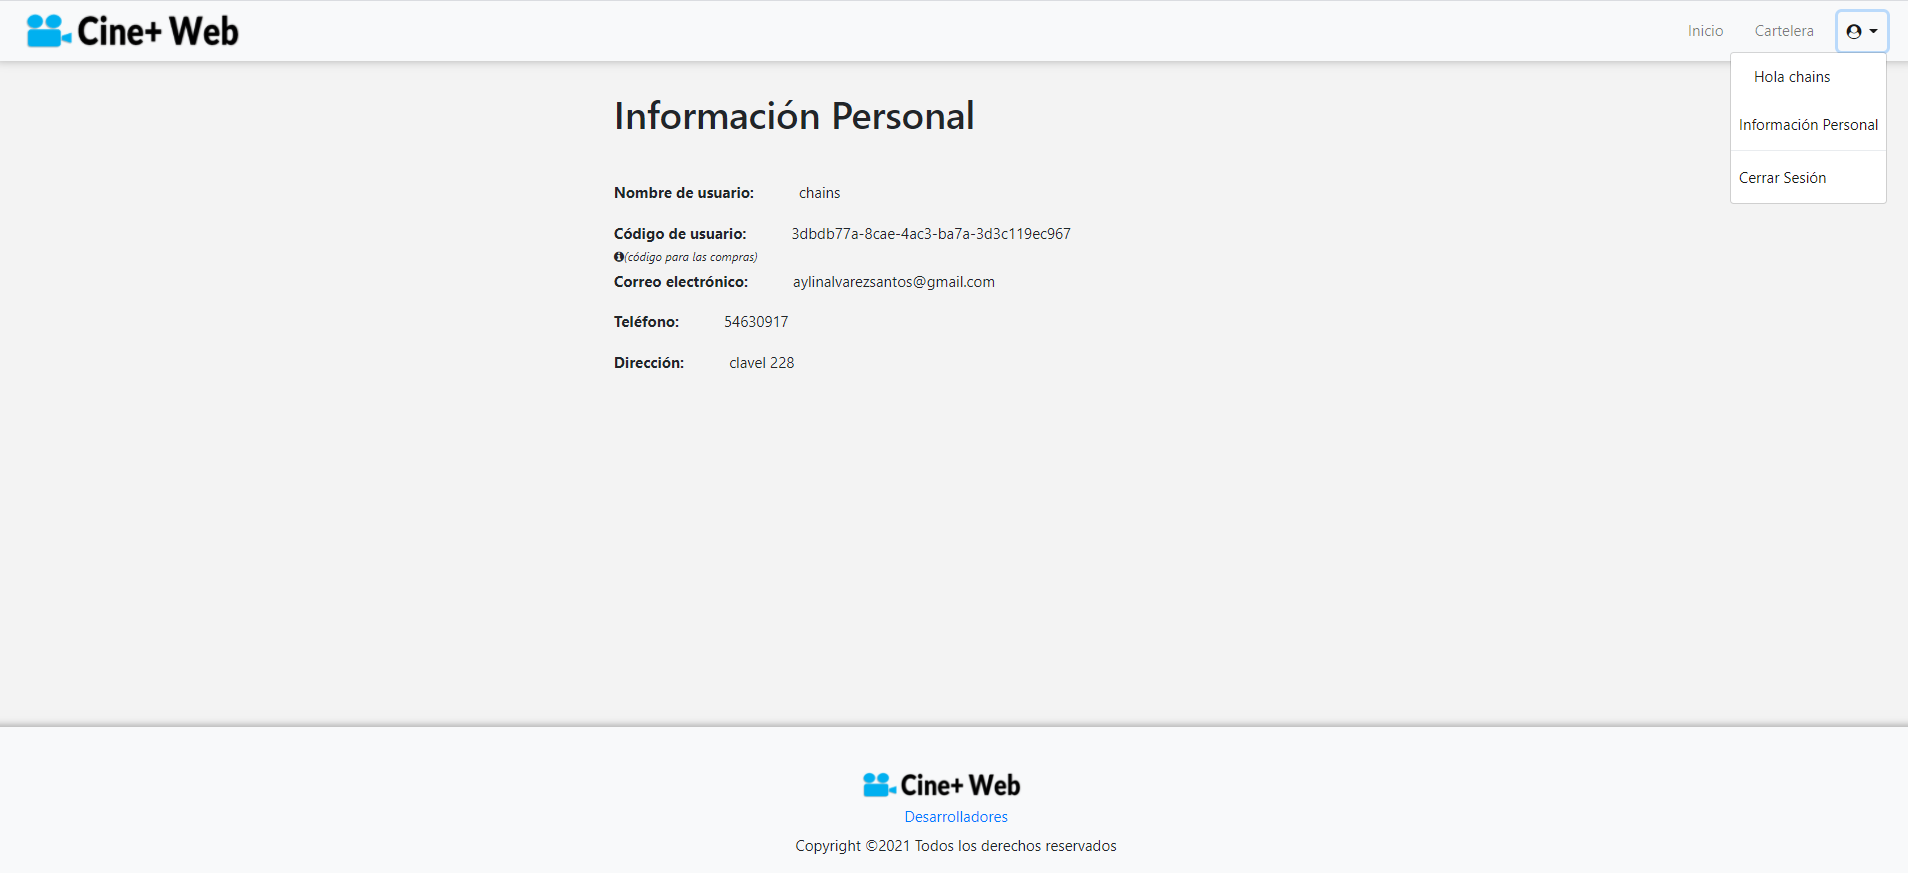
\includegraphics[scale=0.35]{./chapters/img/personal_info.png}
	
	\label{fig:personal_info}
	\caption{Informaci\'on Personal}
	
\end{figure}
\backmatter

% bibliography, glossary and index would go here.

\end{document}